%definira klasu dokumenta 
\documentclass[12pt]{report} 

%prostor izmedu naredbi \documentclass i \begin{document} se zove uvod. U njemu se nalaze naredbe koje se odnose na cijeli dokument

%osnovni LaTex ne može riješiti sve probleme, pa se koriste različiti paketi koji olakšavaju izradu željenog dokumenta
\usepackage[utf8]{inputenc}
%\usepackage[T1]{fontenc}
\usepackage[croatian]{babel} 
\usepackage{amssymb}
\usepackage{amsmath}
\usepackage{txfonts}
\usepackage{mathdots}
\usepackage{titlesec}
\usepackage{array}
\usepackage{lastpage}
\usepackage{etoolbox}
\usepackage{tabularray}
\usepackage{color, colortbl}
\usepackage{adjustbox}
\usepackage{geometry}
\usepackage[classicReIm]{kpfonts}
\usepackage{hyperref}
\usepackage{fancyhdr}

\usepackage{float}
\usepackage{setspace}
\restylefloat{table}
\usepackage{ragged2e}

\usepackage{comment}


\patchcmd{\chapter}{\thispagestyle{plain}}{\thispagestyle{fancy}}{}{} %redefiniranje stila stranice u paketu fancyhdr

%oblik naslova poglavlja
\titleformat{\chapter}{\normalfont\huge\bfseries}{\thechapter.}{20pt}{\Huge}
\titlespacing{\chapter}{0pt}{0pt}{40pt}


\linespread{1.3} %razmak između redaka

\geometry{a4paper, left=1in, top=1in,}  %oblik stranice

\hypersetup{ colorlinks, citecolor=black, filecolor=black, linkcolor=black,	urlcolor=black }   %izgled poveznice


%prored smanjen između redaka u nabrajanjima i popisima
\newenvironment{packed_enum}{
	\begin{enumerate}
		\setlength{\itemsep}{0pt}
		\setlength{\parskip}{0pt}
		\setlength{\parsep}{0pt}
	}{\end{enumerate}}

\newenvironment{packed_item}{
	\begin{itemize}
		\setlength{\itemsep}{0pt}
		\setlength{\parskip}{0pt}
		\setlength{\parsep}{0pt}
	}{\end{itemize}}




%boja za privatni i udaljeni kljuc u tablicama
\definecolor{LightBlue}{rgb}{0.9,0.9,1}
\definecolor{LightGreen}{rgb}{0.9,1,0.9}

%Promjena teksta za dugačke tablice
\DefTblrTemplate{contfoot-text}{normal}{Nastavljeno na idućoj stranici}
\SetTblrTemplate{contfoot-text}{normal}
\DefTblrTemplate{conthead-text}{normal}{(Nastavljeno)}
\SetTblrTemplate{conthead-text}{normal}
\DefTblrTemplate{middlehead,lasthead}{normal}{Nastavljeno od prethodne stranice}
\SetTblrTemplate{middlehead,lasthead}{normal}

%podesavanje zaglavlja i podnožja

\pagestyle{fancy}
\lhead{Programsko inženjerstvo}
\rhead{ConnectiNET}
\lfoot{Eventovci}
\cfoot{stranica \thepage/\pageref{LastPage}}
\rfoot{\today}
\renewcommand{\headrulewidth}{0.2pt}
\renewcommand{\footrulewidth}{0.2pt}


\begin{document} 
	
	
	
	\begin{titlepage}
		\begin{center}
			\vspace*{\stretch{1.0}} %u kombinaciji s ostalim \vspace naredbama definira razmak između redaka teksta
			\LARGE Programsko inženjerstvo\\
			\large Ak. god. 2023./2024.\\
			
			\vspace*{\stretch{3.0}}
			
			\huge ConnectiNET\\
			\Large Dokumentacija, Rev. 1\\
			
			\vspace*{\stretch{12.0}}
			\normalsize
			Grupa: \textit{Eventovci}\\
			Voditelj: \textit{Lucija Topolko}\\
			
			
			\vspace*{\stretch{1.0}}
			Datum predaje: 17. studenog 2023.\\
	
			\vspace*{\stretch{4.0}}
			
			Nastavnik: \textit{dr.sc. Nikolina Frid}\\
		
		\end{center}

	
	\end{titlepage}

	
	\tableofcontents


	\chapter{Dnevnik promjena dokumentacije}
			
		\begin{longtblr}[
				label=none
			]{
				width = \textwidth, 
				colspec={|X[2]|X[13]|X[3]|X[3]|}, 
				rowhead = 1
			}
			\hline
			\textbf{Rev.}	& \textbf{Opis promjene/dodatka} & \textbf{Autori} & \textbf{Datum}\\[3pt] \hline
			0.1 & Napravljen predložak	& Kolarec & 21.10.2023. 		\\[3pt] \hline 
			0.2	& Dodani funkcionalni zahtjevi (3.1 i 3.1.1) & Kolarec & 26.10.2023. \\[3pt] \hline 
			0.3  & Dovršeni funkcionalni zahtjevi (3.1.2 i 3.2) & Kolarec & 31.10.2023.  \\[3pt] \hline
			0.4  & Napisan opis projektnog zadatka & Topolko & 31.10.2023.  \\[3pt] \hline
			0.5 & Dodan opis i dijagrami baze podataka & Kolarec & 2.11.2023.\\[3pt] \hline
			0.6 & Dodan opis arhitekture sustava & Kolarec & 9.11.2023.\\[3pt] \hline
			0.7 & Dodani dijagrami razreda & Kolarec & 12.11.2023. \\[3pt] \hline
			\textbf{1.0} & Dovršena prva verzija dokumentacije & Kolarec &  15.11.2023.\\[3pt] \hline
			 1.1 & Dodan dijagram aktivnosti & Kolarec & 14.12.2023.\\[3pt] \hline
			 1.2 & Dodan dijagram stanja & Kolarec & 18.12.2023. \\[3pt] \hline
			 1.3 & Dodane korištene tehnologije i alati & Topolko & 22.12.2023. \\[3pt] \hline
			 1.4 & Dovršena konačna verzija dijagrama razreda & Kolarec &  2.1.2024.\\[3pt] \hline
			 1.5 & Dodan dijagram komponenti & Kolarec &  10.1.2024 \\[3pt] \hline
			 1.6 & Dodano ispitivanje programskog rješenja & Svalina & 14.1.2024.\\[3pt] \hline
			 & &  & \\[3pt] \hline
			 & &  & \\[3pt] \hline
			 & &  & \\[3pt] \hline
			 & &  & \\[3pt] \hline
			& & & \\[3pt] \hline			
		\end{longtblr}
	

	\chapter{Opis projektnog zadatka}
				
		\section{Uvod}
		
			Cilj ovog projektnog zadatka razviti je programsku potporu za web aplikaciju $\textit{Connectima}$ koja predstavlja inovativnu platformu za promociju raznih vrsta događanja. Aplikacija je namijenjena široj populaciji koja je zainteresirana za najavljena događanja u svojoj okolini ili želi popularizirati svoje događanje. \\ Korisnici mogu pregledavati događanja i njihove organizatore te po završetku događanja iste recenzirati. Također, organizatori događanja mogu ih objavljivati uz mogućnost dodavanja širokog spektra informacija i medijskih sadržaja.\\
			U nastavku su opisani korisnički zahtjevi i glavne funkcionalnosti ove web-aplikacije.
		
		
		
		\section{Opis funkcionalnosti}
		
			\subsection{Stranice}
			
				\subsubsection{Početna stranica}
				Pri pokretanju web aplikacije prikazuje se početna stranica. S lijeve strane stranice nalazi se navigacijska traka s različitim stranicama koje sadrže događanja, podatke o korisniku i drugo. Pošto korisnik u tom trenutku još nije autoriziran, ne može pristupiti nijednoj od dolje navedenih stranica, osim 'Prijava' i 'O nama'.
				
				\subsubsection{O nama}
				Stranica 'O nama' javno je dostupna svima, a ukratko predstavlja cilj web aplikacije i osnovne informacije.
				
				\subsubsection{Prijava}
				 Na stranici prijava korisniku se omogućuje prijava u sustav pomoću adrese elektroničke pošte i lozinke. Ako korisnik još nije registriran u sustav, na istoj se stranici može registrirati i odabrati želi li biti organizator ili posjetitelj. Prijavljeni korisnik neće moći pristupiti ovoj stranici, već će umjesto nje imati mogućnost odjave.
				 
				\subsubsection{Događanja}
				Nakon uspješne prijave ili registracije, korisnika se preusmjeruje na stranicu s događanjima. Može ih filtrirati po vremenu održavanja te otvarati pojedina događanja kako bi dobio više informacija.\\
				Pri pregledu svih događanja prikazuju se naziv događanja, jedna slika, lokacija, vrijeme i organizator, a pri pregledu pojedinačnih događanja prikazuju se svi podaci uključujući organizatora čijim se podacima također može pristupiti.
				
				\subsubsection{Moj račun}
				Na stranici 'Moj račun' korisnik može pregledati i uređivati osobne podatke. Osim navedenog, korisnici koji imaju ovlasti organizatora mogu platiti članarinu. Administrator preko ove stranice može pristupiti popisu svih korisnika te upravljati njima i njihovim događanjima. Posjetitelji i organizatori mogu se pretplatiti na obavijesti za nova događanja po kategoriji ili lokaciji.
				
				\subsubsection{Moja događanja}
				Stranica 'Moja događanja' namijenjena je organizatorima. Na njoj se prikazuju sva događanja koja je organizirao te može njima upravljati ili ih obrisati.
				
				\subsubsection{Moji interesi}
				'Moji interesi' je stranica na kojoj posjetitelji i organizatori mogu lako pronaći događanja za koja su iskazali interes u kategorijama \textit{sigurno dolazim}, \textit{možda dolazim} i \textit{ne dolazim}.
				
				\subsubsection{Inbox}
				Korisnici koji su se pretplatili na obavijesti ovdje će moći vidjeti sva novoobjavljena događanja koja odgovaraju njihovim preferencijama. \\ \\
				
			
			\subsection{Vrste korisnika}
			U sustavu postoje četiri vrste korisnika:
			\begin{packed_enum}
				\item anonimni (neregistrirani) korisnik,
				\item posjetitelj,
				\item organizator i 
				\item administrator.
			\end{packed_enum}
			
			\underline{Anonimni korisnik} ne može koristiti aplikaciju niti pregledavati njen sadržaj dok god se ne prijavi ili registrira. Može se samo upoznati sa izgledom početne stranice i pročitati osnovne informacije o aplikaciji. \\
			
			\underline{Posjetitelj} može pregledati događanja objavljena na stranici, detalje o njima i njihovim organizatorima. Može ih filtrirati po odabranom vremenskom razdoblju (24h, 7 dana, 30 dana, prošla događanja). Također, može pregledati i mijenjati osobne podatke, odjaviti se i obrisati svoj korisnički račun. Na zasebnoj stranici može pregledati događanja za koja je izrazio interes (najavio dolazak). Najaviti dolazak može za bilo koje događanje koje još nije počelo. Po završetku događanja, u roku 48 sati može ostaviti recenziju događanja. Posjetitelj također može uključiti primanje obavijesti o događanjima na nekom području ili neke određene vrste. \\
			
			\underline{Organizator} ima sve ovlasti posjetitelja. Uz to, može dodavati događanja i uređivati ih. Ne može recenzirati vlastita događanja ili najaviti dolazak na njih, ali oni mu se automatski prikazuju u kalendaru.\\
			Postoje dvije skupine organizatora: oni koji aplikaciju koriste besplatno te oni koji plaćaju članarinu. Prema osnovnim postavkama, svaki organizator na početku aplikaciju koristi besplatno. Članarinu mora platiti ako želi dodavati događanja koja nisu besplatna, već se za njih mora platiti ulaznica. \\
			
			\underline{Administrator} ima najveće ovlasti. Njegov je zadatak nadziranje podataka koji se dijele u aplikaciji, dakle događanja i korisnike. Administrator može pregledavati sve korisnike te ih filtrirati na posjetitelje i organizatore. Može obrisati korisničke račune drugih korisnika, pojedina događanja i recenzije. Postavlja i mijenja cijenu članarine. Administrator ne može obrisati svoj račun, dodavati i recenzirati događanja. 
		
		\section{Slična rješenja}
		
		 Već postoje mnoge aplikacije koje imaju isti ili sličan cilj kao i naša aplikacija. Društvene mreže poput Facebooka omogućavaju dodavanje događanja koja se mogu dijeliti na profilu korisnika. S događanjem mogu se povezati naknadne objave korisnika, lokaciju događaja moguće je vidjeti na karti te se, kao i na našoj stranici, može pronaći sve potrebne informacije o samom događanju, ali i njegovom organizatoru. 
		 
		 \begin{figure}[H]
		 	
\includegraphics[scale=0.7]{slike/Facebook_dogadanja.png}
		 	\centering
		 	\caption{Primjer događanja oglašenog na Facebooku}
		 \end{figure}
		
		Iako naša aplikacija u ovoj fazi još ne posjeduje sve te funkcionalnosti, svakako ima prednosti pred navedenom opcijom na Facebooku. Facebook je društvena mreža kojoj oglašavanje događanja nije primarni cilj. Mnogi korisnici žele pratiti događanja u blizini te ista dodavati bez da pritom kreiraju profil na nekoj društvenoj mreži. Upravo je to prednost naše aplikacije koja služi isključivo za promociju događanja.
				
		Drugi je primjer aplikacija \textit{Meetup}. Meetup je po većini funkcionalnosti vrlo sličan našoj aplikaciji. Događanja se mogu filtrirati po lokaciji i vremenu. Dodatna je funkcionalnost s obzirom na \textit{Cennectimu} mogućnost prijave na događanje. Upravo je u tome ključna razlika između ove dvije aplikacije. \textit{Connectima} je zamišljena kao aplikacija za sve vrste događanja, od malih lokalnih okupljanja do velikih koncerata i konferencija. \textit{Meetup} je, s druge strane, aplikacija specijalizirana za konferencije i radionice koje zahtijevaju raniju najavu.\\
	
		 
		\begin{figure}[H]
			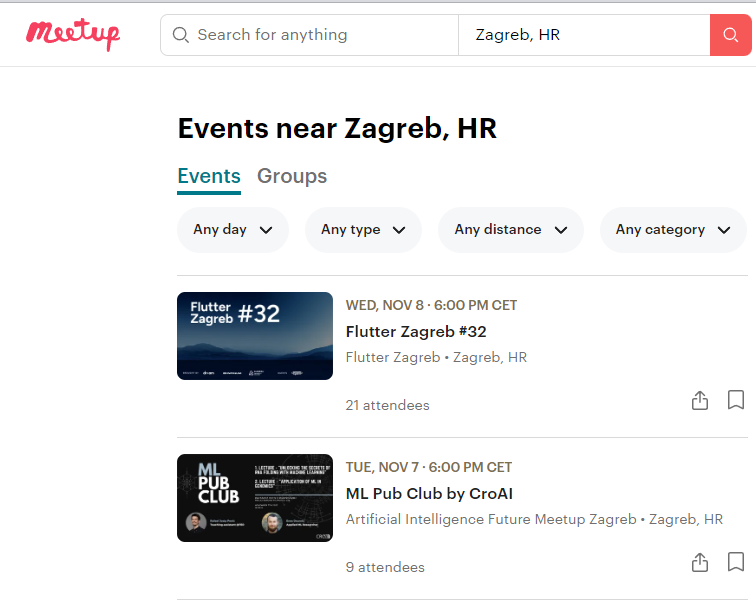
\includegraphics[scale=0.9]{slike/Meetup.png}
			\centering
			\caption{Početna stranica aplikacije Meetup}
		\end{figure}
		
		\newpage
		
		\section{Moguće nadogradnje}
		
		Ova aplikacija ima još puno prostora za nadogradnju pa bi iduće verzije mogle uključivati:
			
			\begin{packed_enum}
				\item uvođenje dodatnih jezika aplikacije (engleski, njemački...),
				\item integraciju s popularnim društvenim mrežama i aplikacijama za razmjenu poruka (Facebook, Instagram, Whatsapp, Viber) za jednostavno dijeljenje događanja
				\item dodatne načine plaćanja
				\item umetanje medijskih sadržaja uz recenziju
				\item preuzimanje događanja u vlastiti kalendar u iCal formatu
				\item pretragu događanja na interaktivnoj karti
				\item mogućnost razmjena poruka među korisnicima
			\end{packed_enum}
			
		Uz sve navedeno, dodatne bi se funkcionalnosti mogle dodavati na temelju povratnih informacija svih korisnika (posjetitelja, organizatora i administratora).
		
		\eject
		
	
	\chapter{Specifikacija programske potpore}

\section{Funkcionalni zahtjevi}

\noindent \textbf{Dionici:}

\begin{packed_enum}
	
	\item Administrator
	\item Organizatori događaja
	\item Građani (posjetitelji)
	\item Razvojni tim				
	
\end{packed_enum}

\noindent \textbf{Aktori i njihovi funkcionalni zahtjevi:}


\begin{packed_enum}
	\item  \underbar{Neregistrirani/neprijavljeni korisnik (inicijator) može:}
	
	\begin{packed_enum}
		\item pregledati stranicu \textit{O nama}
		\item stvoriti novi korisnički račun kao:
		\begin{packed_enum}
			\item organizator (korisničko ime, e-mail adresa, lozinka, adresa) 
			\item  posjetitelj (korisničko ime, e-mail adresa, lozinka) 
		\end{packed_enum} 
		\item prijaviti se u sustav
		
	\end{packed_enum}
	
	\item  \underbar{Posjetitelj (inicijator) može:}
	
	\begin{packed_enum}
		
		\item prijaviti se u sustav i odjaviti iz sustava
		\item pregledavati i uređivati svoje osobne podatke
		\item vidjeti popis aktualnih događanja u odabranom vremenskom razdoblju (24 sata, 7 dana, 30 dana)
		\item odabrati postavke da im aplikacija automatski šalje obavijesti o najnovijim događanjima (prema vrsti događanja i području) 
		\item za svako događanje: 
		\begin{packed_enum}
			\item iskazati interes (\textit{sigurno dolazim, možda dolazim, ne dolazim})
			\item po želji promijeniti interes
		\end{packed_enum} 
		\item vidjeti podatke o organizatorima događanja (naziv, adresa, poveznica na vlastite web ili Facebook stranice,  popis svih događanja koja su oglašena putem aplikacije u zadnje 2 godine)
		\item napisati recenziju (i/ili obrisati svoju napisanu recenziju) za događanja koja su završila u posljednjih 48 sati
		\item obrisati svoj korisnički račun
		\item odjaviti se iz sustava
		
	\end{packed_enum}
	
	\item \underbar{Organizator (inicijator) može:}		
	
	\begin{packed_enum}
		\item sve što može i Posjetitelj
		\item unošenjem obaveznih i, po želji, opcionalnih podataka, ovisno plaća li članarinu, stvoriti novo događanje:
		\begin{packed_enum}
			\item za koje se ne plaća ulaz 
			\item za koje se plaća ulaz ili za koje se ne plaća ulaz
		\end{packed_enum}
		\item pregledavati i brisati svoja događanja 
	\end{packed_enum}
	
	\item \underbar{Administrator (inicijator) može:}
	
	\begin{packed_enum}
		\item prijaviti se u sustav
		\item vidjeti popis i osobne podatke svih registriranih korisnika 
		\item trajno obrisati korisnički profil
		\item postaviti cijenu članarine za organizatore događanja za koje se plaća ulaz
		\item brisati recenzije i događanja 
		\item odjaviti se iz sustava
	\end{packed_enum}
	
	\item \underbar{Baza podataka (sudionik):}
	\begin{packed_enum}
		\item pohranjuje podatke registriranih korisnika 
		\item pohranjuje podatke o događanjima 
		\item pohranjuje recenzije događanja 
	\end{packed_enum}
\end{packed_enum}

\eject 



\subsection{Obrasci uporabe}

\subsubsection{Opis obrazaca uporabe}

\noindent U nastavku su detaljno opisani obrasci upotrebe označenih kraticom UC i rednim brojem obrasca. Obrasci predstavljaju ključne scenarije interakcije između korisnika i samog sustava. Svaki UC pruža jasno strukturirane korake koje korisnik slijedi i omogućuje razumijevanje odziva sustava na te korake.  \\

\noindent \underbar{\textbf{UC1 - Pregled stranice O nama}}
\begin{packed_item}
	
	\item \textbf{Glavni sudionik:} Neregistrirani/neprijavljeni korisnik i prijavljeni korisnik
	\item  \textbf{Cilj:} Pregled stranice s općim informacijama o web aplikaciji
	\item  \textbf{Sudionici:} -
	\item  \textbf{Preduvjet:} -
	\item  \textbf{Opis osnovnog tijeka:}
	
	\item[] \begin{packed_enum}
		
		\item Korisnik odabire opciju prikaza stranice O nama
		\item Otvara se stranica i prikazuju informacije o web aplikaciji
		
	\end{packed_enum}						
\end{packed_item}


%	%	%	%	%	%	%	%	%	%	%	%	%	%	%	%	%					

\noindent \underbar{\textbf{UC2 - Registracija}}
\begin{packed_item}
	
	\item \textbf{Glavni sudionik:} Neregistrirani/neprijavljeni korisnik
	\item  \textbf{Cilj:} Stvaranje korisničkog računa za korištenje platforme
	\item  \textbf{Sudionici:} Baza podataka
	\item  \textbf{Preduvjet:} -
	\item  \textbf{Opis osnovnog tijeka:}
	
	\item[] \begin{packed_enum}
		
		\item Korisnik odabire opciju registracije
		\item Korisnik unosi tražene podatke 
		\item Baza podataka se osvježava
		\item Korisnik dobiva pristup korisničkim funkcijama i obavijest o uspješnoj registraciji te se preusmjerava na početnu stranicu za prijavljene korisnike 
		
	\end{packed_enum}
	
	\item  \textbf{Opis mogućih odstupanja:}
	
	\item[] \begin{packed_item}
		
		\item[2.a] Uneseno zauzeto korisničko ime i/ili e-mail adresa, korisničko ime i/ili lozinka u nedozvoljenom formatu, neispravna e-mail adresa 
		\item[] \begin{packed_enum}
			
			\item Obavijestiti korisnika o neispravnom unosu i omogućiti ponovni unos neprihvaćenih vrijednosti
			\item Korisnik unosi nove vrijednosti i uspješno završava registraciju ili odustaje od registracije 
			
		\end{packed_enum}
	\end{packed_item}
	
\end{packed_item}

%	%	%	%	%	%	%	%	%	%	%	%	%	%	%	%	%	%	%

\newpage

\noindent \underbar{\textbf{UC3 - Prijava}}
\begin{packed_item}
	
	\item \textbf{Glavni sudionik:} Neregistrirani/neprijavljeni korisnik
	\item  \textbf{Cilj:} Dobiti pristup odgovarajućem korisničkom sučelju ovisno o ulozi 
	\item  \textbf{Sudionici:} Baza podataka
	\item  \textbf{Preduvjet:} Registracija
	\item  \textbf{Opis osnovnog tijeka:}
	
	\item[] \begin{packed_enum}
		
		\item Korisnik odabire opciju prijave u sustav
		\item Korisnik unosi tražene podatke (korisničko ime i lozinka)
		\item Provjera ispravnosti unesenih podataka 
		\item Korisnik dobiva obavijest o uspješnoj prijavi i preusmjerava se na početnu stranicu za prijavljene korisnike 
		
	\end{packed_enum}
	
	\item  \textbf{Opis mogućih odstupanja:}
	
	\item[] \begin{packed_item}
		
		\item[2.a] Uneseno neispravno korisničko ime i/ili lozinka  
		\item[] \begin{packed_enum}
			
			\item Obavijestiti korisnika o neuspješnoj registraciji i omogućiti ponovni unos korisničkog imena i/ili lozinke
			\item Korisnik unosi nove vrijednosti i uspješno se prijavljuje ili odustaje od prijave
			
		\end{packed_enum}
	\end{packed_item}
	
\end{packed_item}

%	%	%	%	%	%	%	%	%	%	%	%	%	%	%	%	%	%	%


\noindent \underbar{\textbf{UC4 - Odjava}}
\begin{packed_item}
	
	\item \textbf{Glavni sudionik:} Prijavljeni korisnik (Administrator, Organizator, Posjetitelj)
	\item  \textbf{Cilj:} Odjava iz sustava 
	\item  \textbf{Sudionici:} -
	\item  \textbf{Preduvjet:} Korisnik je trenutno prijavljen u sustav
	\item  \textbf{Opis osnovnog tijeka:}
	
	\item[] \begin{packed_enum}
		
		\item Korisnik odabire opciju odjave
		\item Korisnik gubi pristup korisničkim funkcijama
		\item Korisnik se preusmjerava na početnu stranicu za neregistrirane/neprijavljene korisnike 
		
	\end{packed_enum}
\end{packed_item}

%	%	%	%	%	%	%	%	%	%	%	%	%	%	%	%	%	%	%

\noindent \underbar{\textbf{UC5 - Pregled osobnih podataka}}
\begin{packed_item}
	
	\item \textbf{Glavni sudionik:} Korisnik (Organizator, Posjetitelj)
	\item  \textbf{Cilj:} Pregledati osobne podatke
	\item  \textbf{Sudionici:} Baza podataka
	\item  \textbf{Preduvjet:} Korisnik je trenutno prijavljen u sustav
	\item  \textbf{Opis osnovnog tijeka:}
	
	\item[] \begin{packed_enum}
		
		\item Korisnik odabire opciju za pregled svog profila
		\item Prikazuju se osobni podaci vezani uz korisnički račun
		
	\end{packed_enum}
\end{packed_item}

%	%	%	%	%	%	%	%	%	%	%	%	%	%	%	%	%	%	%

\noindent \underbar{\textbf{UC6 - Uređivanje osobnih podataka}}
\begin{packed_item}
	
	\item \textbf{Glavni sudionik:} Korisnik (Organizator, Posjetitelj)
	\item  \textbf{Cilj:} Izmijeniti osobne podatke 
	\item  \textbf{Sudionici:} Baza podataka
	\item  \textbf{Preduvjet:} Korisnik je trenutno prijavljen u sustav
	\item  \textbf{Opis osnovnog tijeka:}
	
	\item[] \begin{packed_enum}
		
		\item Korisnik odabire opciju izmjene osobnih podataka
		\item Korisnik mijenja željene podatke 
		\item Provjera ispravnosti unesenih podataka 
		\item Korisnik sprema promjene
		\item Baza podataka se osvježava 
		
	\end{packed_enum}
	
	\item  \textbf{Opis mogućih odstupanja:}
	
	\item[] \begin{packed_item}
		
		\item[2.a] Novo uneseni podaci su nedozvoljene vrijednosti
		\item[] \begin{packed_enum}
			
			\item Onemogućiti spremanje promjena
			\item Obavijestiti korisnika o nedozvoljenim vrijednostima i omogućiti ponovni unos 
			\item Korisnik unosi nove vrijednosti i omogućava se spremanje promjena
			
		\end{packed_enum}
		
		\item[4.a] Korisnik pokušava napustiti prozor, a nije spremio promjene 
		\item[] \begin{packed_enum}
			
			\item Obavijestiti korisnika o obaveznom spremanju promjena
			\item Nakon spremanja promjena omogućiti izlaz iz prozora
			
		\end{packed_enum}
		
	\end{packed_item}
	
\end{packed_item}

%	%	%	%	%	%	%	%	%	%	%	%	%	%	%	%	%	%	%

\noindent \underbar{\textbf{UC7 - Postavke obavještavanja o novim događanjima}}
\begin{packed_item}
	
	\item \textbf{Glavni sudionik:} Prijavljeni korisnik (Organizator, Posjetitelj)
	\item  \textbf{Cilj:} Podesiti postavke obavještavanja o najnovijim događanjima
	\item  \textbf{Sudionici:} Baza podataka
	\item  \textbf{Preduvjet:} Korisnik je trenutno prijavljen u sustav i ima ovlasti Posjetitelja
	\item  \textbf{Opis osnovnog tijeka:}
	
	\item[] \begin{packed_enum}
		
		\item Korisnik odabire opciju uređivanja postavki obavještavanja o novim događanjima
		\item Korisnik odabire želi li primati obavijesti i, ako da, o kojim vrstama događanja i na kojem području
		\item Korisnik sprema promjene
		\item Baza podataka se osvježava
		
	\end{packed_enum}
	
	%\item  \textbf{Opis mogućih odstupanja:}
	
	%\item[] \begin{packed_item}
		
		%	\item[2.a] Korisnik odabire da želi primati obavijesti, ali ne unese minimalno jednu vrstu događanja i minimalno jedno područje
		%	\item[] \begin{packed_enum}
			
			%		\item Onemogućiti spremanje promjena
			%		\item Obavijestiti korisnika o obaveznom izboru barem jedne vrste događanja i barem jednog područja
			%		\item Korisnik odabire vrstu događanja i/ili područje koje nedostaje i omogućava se spremanje promjena
			
			%	\end{packed_enum}
		%\end{packed_item}
		
	\end{packed_item}
	
	%	%	%	%	%	%	%	%	%	%	%	%	%	%	%	%	%	%	%
	
	\noindent \underbar{\textbf{UC8 - Brisanje vlastitog korisničkog računa}}
	\begin{packed_item}
		
		\item \textbf{Glavni sudionik:} Korisnik (Organizator, Posjetitelj)
		\item  \textbf{Cilj:} Obrisati korisnički račun i sve osobne podatke
		\item  \textbf{Sudionici:} Baza podataka
		\item  \textbf{Preduvjet:} Korisnik je trenutno prijavljen u sustav i otvoren je pregled osobnih podataka
		\item  \textbf{Opis osnovnog tijeka:}
		
		\item[] \begin{packed_enum}
			
			\item Korisnik odabire opciju brisanja korisničkog računa
			\item Korisnik potvrđuje svoj odabir 
			\item Baza podataka se osvježava
			\item Korisnik se preusmjerava na početnu stranicu za neregistrirane/neprijavljene korisnike 
			
		\end{packed_enum}
		
	\end{packed_item}
	
	%	%	%	%	%	%	%	%	%	%	%	%	%	%	%	%	%	%	%
	
	
	\noindent \underbar{\textbf{UC9 - Pregled svih korisničkih računa}}
	\begin{packed_item}
		
		\item \textbf{Glavni sudionik:} Administrator
		\item  \textbf{Cilj:} Prikaz svih korisničkih računa 
		\item  \textbf{Sudionici:} Baza podataka
		\item  \textbf{Preduvjet:} Korisnik je trenutno prijavljen u sustav i ima ovlasti Administratora
		\item  \textbf{Opis osnovnog tijeka:}
		
		\item[] \begin{packed_enum}
			
			\item Administrator odabire opciju pregleda korisničkih računa
			\item Prikazuje se popis svih korisničkih računa
			
		\end{packed_enum}
		
	\end{packed_item}
	
	%	%	%	%	%	%	%	%	%	%	%	%	%	%	%	%	%	%	%
	
	\noindent \underbar{\textbf{UC10 - Brisanje korisničkog računa}}
	\begin{packed_item}
		
		\item \textbf{Glavni sudionik:} Administrator
		\item  \textbf{Cilj:} Trajno brisanje korisnika iz sustava
		\item  \textbf{Sudionici:} Baza podataka
		\item  \textbf{Preduvjet:} Korisnik je prijavljen, ima ovlasti Administratora i prikazan mu je popis svih korisničkih računa (\textbf{UC9})
		\item  \textbf{Opis osnovnog tijeka:}
		
		\item[] \begin{packed_enum}
			
			\item Administrator odabire opciju brisanja korisničkog računa 
			\item Administrator potvrđuje svoj odabir
			\item Baza podataka se osvježava
			\item Promjena je vidljiva u prikazanom popisu korisničkih računa
			
		\end{packed_enum}
		
	\end{packed_item}
	
	%	%	%	%	%	%	%	%	%	%	%	%	%	%	%	%	%	%	%
	
	\newpage
	
	\noindent \underbar{\textbf{UC11 - Postavljanje cijene članarine}}
	\begin{packed_item}
		
		\item \textbf{Glavni sudionik:} Administrator
		\item  \textbf{Cilj:} Postavljanje cijene mjesečne članarine za organizatore
		\item  \textbf{Sudionici:} Baza podataka
		\item  \textbf{Preduvjet:} Korisnik je prijavljen i ima ovlasti Administratora 
		\item  \textbf{Opis osnovnog tijeka:}
		
		\item[] \begin{packed_enum}
			
			\item Administrator odabire opciju postavljanja članarine
			\item Administrator unosi cijenu i sprema ju
			\item Baza podataka se osvježava
			
		\end{packed_enum}
		
		\item  \textbf{Opis mogućih odstupanja:}
		
		\item[] \begin{packed_item}
			
			\item[2.a] Unesena cijena nije ispravnog formata
			\item[] \begin{packed_enum}
				
				\item Onemogućiti spremanje promjena
				\item Obavijestiti korisnika o nedozvoljenoj vrijednosti i omogućiti ponovni unos 
				\item Korisnik unosi novu vrijednost i omogućava se spremanje promjena
				
			\end{packed_enum}
		\end{packed_item}
		
	\end{packed_item}
	
	%	%	%	%	%	%	%	%	%	%	%	%	%	%	%	%	%	%	%
	
	\noindent \underbar{\textbf{UC12 - Dodavanje novog događanja}}
	\begin{packed_item}
		
		\item \textbf{Glavni sudionik:} Organizator
		\item  \textbf{Cilj:} Dodati novo događanje 
		\item  \textbf{Sudionici:} Baza podataka
		\item  \textbf{Preduvjet:} Korisnik je prijavljen i ima ovlasti Organizatora
		\item  \textbf{Opis osnovnog tijeka:}
		
		\item[] \begin{packed_enum}
			
			\item Organizator odabire opciju dodavanja novog događanja
			\item Organizator upisuje potrebne i, po želji, opcionalne podatke o događanju (naziv, vrsta, lokacija, vrijeme početka, trajanje, cijena; opcionalno fotografije, videozapisi)
			
			\item Ovisno o tome ima li Organizator mogućnost organiziranja događanja koja se plaćaju: 
			\item[] \begin{packed_enum}
				\item ako ima, Organizator bira plaća li se ili ne novo događanje koje dodaje 
				\item ako nema mogućnost organiziranja događanja koja se plaćaju, podrazumijeva se da je događanje besplatno
			\end{packed_enum}
			
			\item Organizator dovršava objavu i objavljuje ju
			\item Baza podataka se osvježava
			\item Događanje će biti prikazano na stranici
			
		\end{packed_enum}
		
		\item  \textbf{Opis mogućih odstupanja:}
		
		\item[] \begin{packed_item}
			
			\item[2.a] Uneseni podaci su nedozvoljene vrijednosti
			\item[] \begin{packed_enum}
				
				\item Onemogućiti završetak dodavanja događanja
				\item Obavijestiti korisnika o nedozvoljenim vrijednostima i omogućiti ponovni unos 
				\item Korisnik unosi nove vrijednosti i omogućava se nastavak na objavu događanja
				
			\end{packed_enum}		
		\end{packed_item}
		
	\end{packed_item}
	
	%	%	%	%	%	%	%	%	%	%	%	%	%	%	%	%	%	%	%
	
	\noindent \underbar{\textbf{UC13 - Pregled svih događanja}}
	\begin{packed_item}
		
		\item \textbf{Glavni sudionik:} Prijavljeni korisnik (Posjetitelj, Organizator, Administrator)
		\item  \textbf{Cilj:} Pregled svih događanja prema određenom kriteriju
		\item  \textbf{Sudionici:} Baza podataka
		\item  \textbf{Preduvjet:} Korisnik je trenutno prijavljen u sustav 
		\item  \textbf{Opis osnovnog tijeka:}
		
		\item[] \begin{packed_enum}
			
			\item Na stranici s događanjima korisnik odabire kriterij prema kojem se prikazuju događanja (prikaz događanja završenih u zadnjih 48 sati ili aktualna događanja u narednih 24 sata, 7 dana, 30 dana)
			\item Događanja koja zadovoljavaju odabrani kriterij prikazuju se na stranici
			
		\end{packed_enum}
		
	\end{packed_item}
	
	%	%	%	%	%	%	%	%	%	%	%	%	%	%	%	%	%	%	%
	
	\noindent \underbar{\textbf{UC14 - Pregled jednog događanja}}
	\begin{packed_item}
		
		\item \textbf{Glavni sudionik:} Prijavljeni korisnik (Posjetitelj, Organizator, Administrator)
		\item  \textbf{Cilj:} Pregled jednog odabranog događanja od svih prikazanih događanja 
		\item  \textbf{Sudionici:} Baza podataka
		\item  \textbf{Preduvjet:} Korisnik je trenutno prijavljen u sustav i prikazana su sva događanja prema odabranom kriteriju (\textbf{UC13})
		\item  \textbf{Opis osnovnog tijeka:}
		
		\item[] \begin{packed_enum}
			
			\item Korisnik odabire jedno od prikazanih događanja
			\item Na zasebnoj se stranici korisniku prikazuju detalji o odabranom događanju
			
		\end{packed_enum}
		
	\end{packed_item}
	
	%	%	%	%	%	%	%	%	%	%	%	%	%	%	%	%	%	%	%				
	
	\noindent \underbar{\textbf{UC15 - Pregled profila organizatora}}
	\begin{packed_item}
		
		\item \textbf{Glavni sudionik:} Prijavljeni korisnik (Posjetitelj, Organizator)
		\item  \textbf{Cilj:} Pregled korisničkog računa organizatora
		\item  \textbf{Sudionici:} Baza podataka
		\item  \textbf{Preduvjet:} Korisnik je trenutno prijavljen u sustav, ima ovlasti Posjetitelja ili Organizatora i ima otvoren prikaz nekog događanja
		\item  \textbf{Opis osnovnog tijeka:}
		
		\item[] \begin{packed_enum}
			
			\item Posjetitelj odabire opciju prikaza profila organizatora
			\item Prikazuju se informacije o organizatoru
			
		\end{packed_enum}
		
	\end{packed_item}
	
	%	%	%	%	%	%	%	%	%	%	%	%	%	%	%	%	%	%	%
	
	\noindent \underbar{\textbf{UC16 - Pregled vlastitih događanja}}
	\begin{packed_item}
		
		\item \textbf{Glavni sudionik:} Organizator
		\item  \textbf{Cilj:} Pregled svih događanja koje je taj organizator objavio
		\item  \textbf{Sudionici:} Baza podataka
		\item  \textbf{Preduvjet:} Korisnik je trenutno prijavljen u sustav i ima ovlasti Organizatora  
		\item  \textbf{Opis osnovnog tijeka:}
		
		\item[] \begin{packed_enum}
			
			\item Organizator odabire opciju prikaza vlastitih događanja
			\item Ovisno o tome ima li organizator objavljenih događanja prikazuju se događanja ili odgovarajuća poruka
			
		\end{packed_enum}
		
	\end{packed_item}
	
	%	%	%	%	%	%	%	%	%	%	%	%	%	%	%	%	%	%	%
	
	\noindent \underbar{\textbf{UC17 - Pregled jednog vlastitog događanja}}
	\begin{packed_item}
		
		\item \textbf{Glavni sudionik:} Organizator
		\item  \textbf{Cilj:} Prikaz jednog od događanja koje je taj organizator objavio
		\item  \textbf{Sudionici:} Baza podataka
		\item  \textbf{Preduvjet:} Korisnik je trenutno prijavljen u sustav, ima ovlasti Organizatora i prikazana su mu sva vlastita događanja
		\item  \textbf{Opis osnovnog tijeka:}
		
		\item[] \begin{packed_enum}
			
			\item Organizator odabire opciju prikaza jednog od događanja
			\item Na zasebnoj se stranici organizatoru prikazuju detalji o odabranom događaju (uključujući i recenzije posjetitelja)
			
		\end{packed_enum}
		
	\end{packed_item}
	
	%	%	%	%	%	%	%	%	%	%	%	%	%	%	%	%	%	%	%
	
	\noindent \underbar{\textbf{UC18 - Brisanje vlastitog događanja}}
	\begin{packed_item}
		
		\item \textbf{Glavni sudionik:} Organizator
		\item  \textbf{Cilj:} Trajno brisanje vlastitog događanja
		\item  \textbf{Sudionici:} Baza podataka
		\item  \textbf{Preduvjet:} Korisnik je prijavljen, ima ovlasti Organizatora i prikazana su mu sva vlastita događanja
		\item  \textbf{Opis osnovnog tijeka:}
		
		\item[] \begin{packed_enum}
			
			\item Organizator odabire opciju brisanja događanja
			\item Organizator potvrđuje svoj odabir
			\item Baza podataka se osvježava
			\item Promjena je vidljiva u prikazanom popisu događanja
			
		\end{packed_enum}
		
	\end{packed_item}
	
	%	%	%	%	%	%	%	%	%	%	%	%	%	%	%	%	%	%	%
	
	\noindent \underbar{\textbf{UC19 - Brisanje događanja}}
	\begin{packed_item}
		
		\item \textbf{Glavni sudionik:} Administrator
		\item  \textbf{Cilj:} Trajno brisanje događanja
		\item  \textbf{Sudionici:} Baza podataka
		\item  \textbf{Preduvjet:} Korisnik je prijavljen, ima ovlasti Administratora i prikazana su mu sva događanja
		\item  \textbf{Opis osnovnog tijeka:}
		
		\item[] \begin{packed_enum}
			
			\item Administrator odabire opciju brisanja događanja
			\item Administrator potvrđuje svoj odabir
			\item Baza podataka se osvježava
			\item Promjena je vidljiva u prikazanom popisu događanja
			
		\end{packed_enum}
		
	\end{packed_item}
	
	%	%	%	%	%	%	%	%	%	%	%	%	%	%	%	%	%	%	%
	
	\noindent \underbar{\textbf{UC20 - Recenziranje događanja}}
	\begin{packed_item}
		
		\item \textbf{Glavni sudionik:} Prijavljeni korisnik (Organizator, Posjetitelj)
		\item  \textbf{Cilj:} Dodavanje recenzije događanja
		\item  \textbf{Sudionici:} Baza podataka
		\item  \textbf{Preduvjet:} Korisnik je prijavljen, ima ovlasti Posjetitelja ili Organizatora i otvoren je prikaz događanja koje je završilo u posljednjih 48 sati
		\item  \textbf{Opis osnovnog tijeka:}
		
		\item[] \begin{packed_enum}
			
			\item Posjetitelj odabire opciju dodavanja recenzije
			\item Posjetitelj upisuje ocjenu i recenziju događanja
			\item Posjetitelj potvrđuje da želi objaviti recenziju ili odustaje od objave
			\item Baza podataka se osvježava
			\item Recenzija je dodana i vidljiva na vrhu recenzija tog događanja
			
		\end{packed_enum}
		
		\item  \textbf{Opis mogućih odstupanja:}
		
		\item[] \begin{packed_item}
			
			\item[2.a] Recenzija nije napisana 
			\item[] \begin{packed_enum}
				
				\item Onemogućiti objavu recenzije 
				\item Posjetitelju omogućiti objavu recenzije ako i samo ako recenzija nije prazna, u protivnom posjetitelj odustaje od objave recenzije
				
			\end{packed_enum}		
		\end{packed_item}
		
	\end{packed_item}
	
	%	%	%	%	%	%	%	%	%	%	%	%	%	%	%	%	%	%	%
	
	\newpage
	
	\noindent \underbar{\textbf{UC21 - Brisanje vlastite recenzije}}
	\begin{packed_item}
		
		\item \textbf{Glavni sudionik:} Prijavljeni korisnik (Posjetitelj, Organizator)
		\item  \textbf{Cilj:} Trajno brisanje vlastite recenzije događanja
		\item  \textbf{Sudionici:} Baza podataka
		\item  \textbf{Preduvjet:} Korisnik je prijavljen, ima ovlasti Posjetitelja ili Organizatora i otvoren je prikaz jednog događanja
		\item  \textbf{Opis osnovnog tijeka:}
		
		\item[] \begin{packed_enum}
			
			\item Korisnik odabire opciju brisanja recenzije 
			\item Korisnik potvrđuje svoj odabir
			\item Baza podataka se osvježava
			\item Promjena je vidljiva u prikazanom događanju
			
		\end{packed_enum}
		
	\end{packed_item}
	
	%	%	%	%	%	%	%	%	%	%	%	%	%	%	%	%	%	%	%
	
	\noindent \underbar{\textbf{UC22 - Brisanje recenzije}}
	\begin{packed_item}
		
		\item \textbf{Glavni sudionik:} Administrator
		\item  \textbf{Cilj:} Trajno brisanje recenzije događanja
		\item  \textbf{Sudionici:} Baza podataka
		\item  \textbf{Preduvjet:} Korisnik je prijavljen, ima ovlasti Administratora i otvoren je prikaz jednog događanja
		\item  \textbf{Opis osnovnog tijeka:}
		
		\item[] \begin{packed_enum}
			
			\item Administrator odabire opciju brisanja recenzije 
			\item Administrator potvrđuje svoj odabir
			\item Baza podataka se osvježava
			\item Promjena je vidljiva u prikazanom događanju
			
		\end{packed_enum}
		
	\end{packed_item}
	
	%	%	%	%	%	%	%	%	%	%	%	%	%	%	%	%	%	%	%
	
	
	\noindent \underbar{\textbf{UC23 - Iskazivanje interesa za događanje}}
	\begin{packed_item}
		
		\item \textbf{Glavni sudionik:} Prijavljeni korisnik (Posjetitelj, Organizator)
		\item  \textbf{Cilj:} Izraziti i/ili promijeniti interes za događanje
		\item  \textbf{Sudionici:} Baza podataka
		\item  \textbf{Preduvjet:} Korisnik je trenutno prijavljen u sustav, ima ovlasti Posjetitelja ili Organizatora i otvoren je  prikaz nekog događanja 
		\item  \textbf{Opis osnovnog tijeka:}
		
		\item[] \begin{packed_enum}
			
			\item Posjetitelj odabire jednu od opcija \textit{sigurno dolazim, možda dolazim, ne dolazim }
			\item Eventualnim ponovnim pritiskom na opciju koja je odabrana poništava se taj odabir
			\item Baza podataka se osvježava
			\item Na prikazu tog događanja korisnik vidi svoj zadnji iskazani interes 
			
		\end{packed_enum}
		
		\item  \textbf{Opis mogućih odstupanja:}
		
		\item[] \begin{packed_item}
			
			\item[1.a] Posjetitelj odabire novu opciju, a jedna je već odabrana  
			\item[] \begin{packed_enum}
				
				\item Poništava se odabir koji je do tada vrijedio i bilježi se novi odabir
				
			\end{packed_enum}		
		\end{packed_item}
		
	\end{packed_item}
	
	
	
	\newpage
	
	
	\subsubsection{Dijagrami obrazaca uporabe}
	
	\begin{figure}[H]
		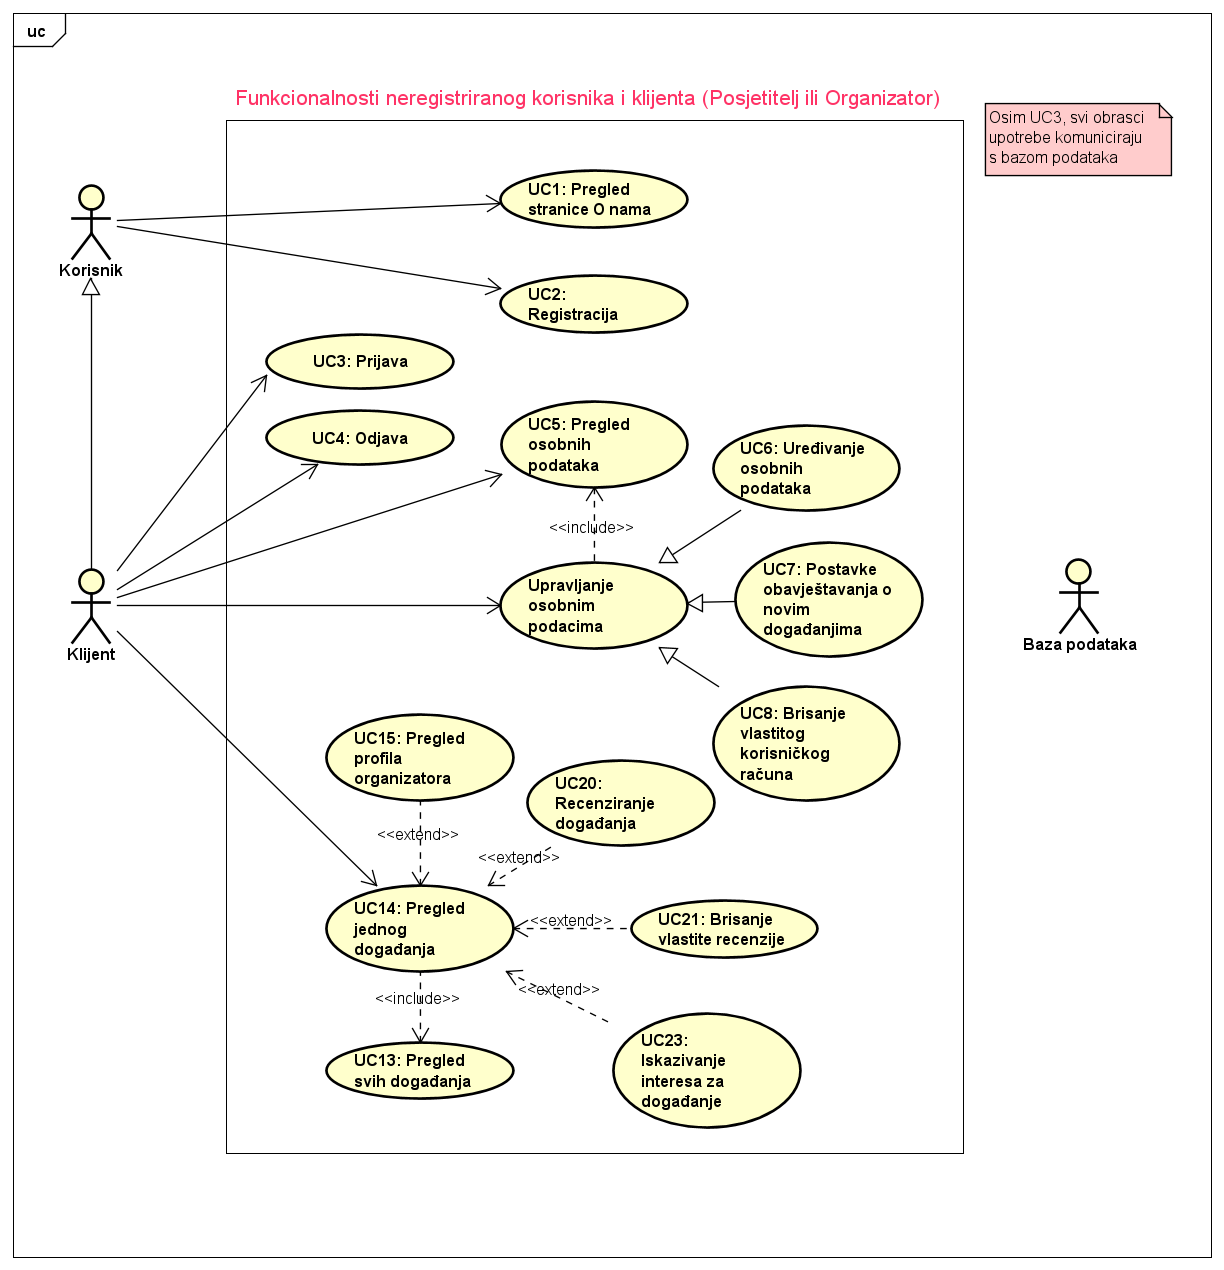
\includegraphics[scale=0.5]{dijagrami/uc1.PNG} 
		\centering
		\caption{Dijagram obrazaca uporabe, funkcionalnost Korisnika i Klijenta (Posjetitelj, Organizator)}
		\label{fig:promjene}
	\end{figure}
	
	\newpage
	
	\begin{figure}[H]
		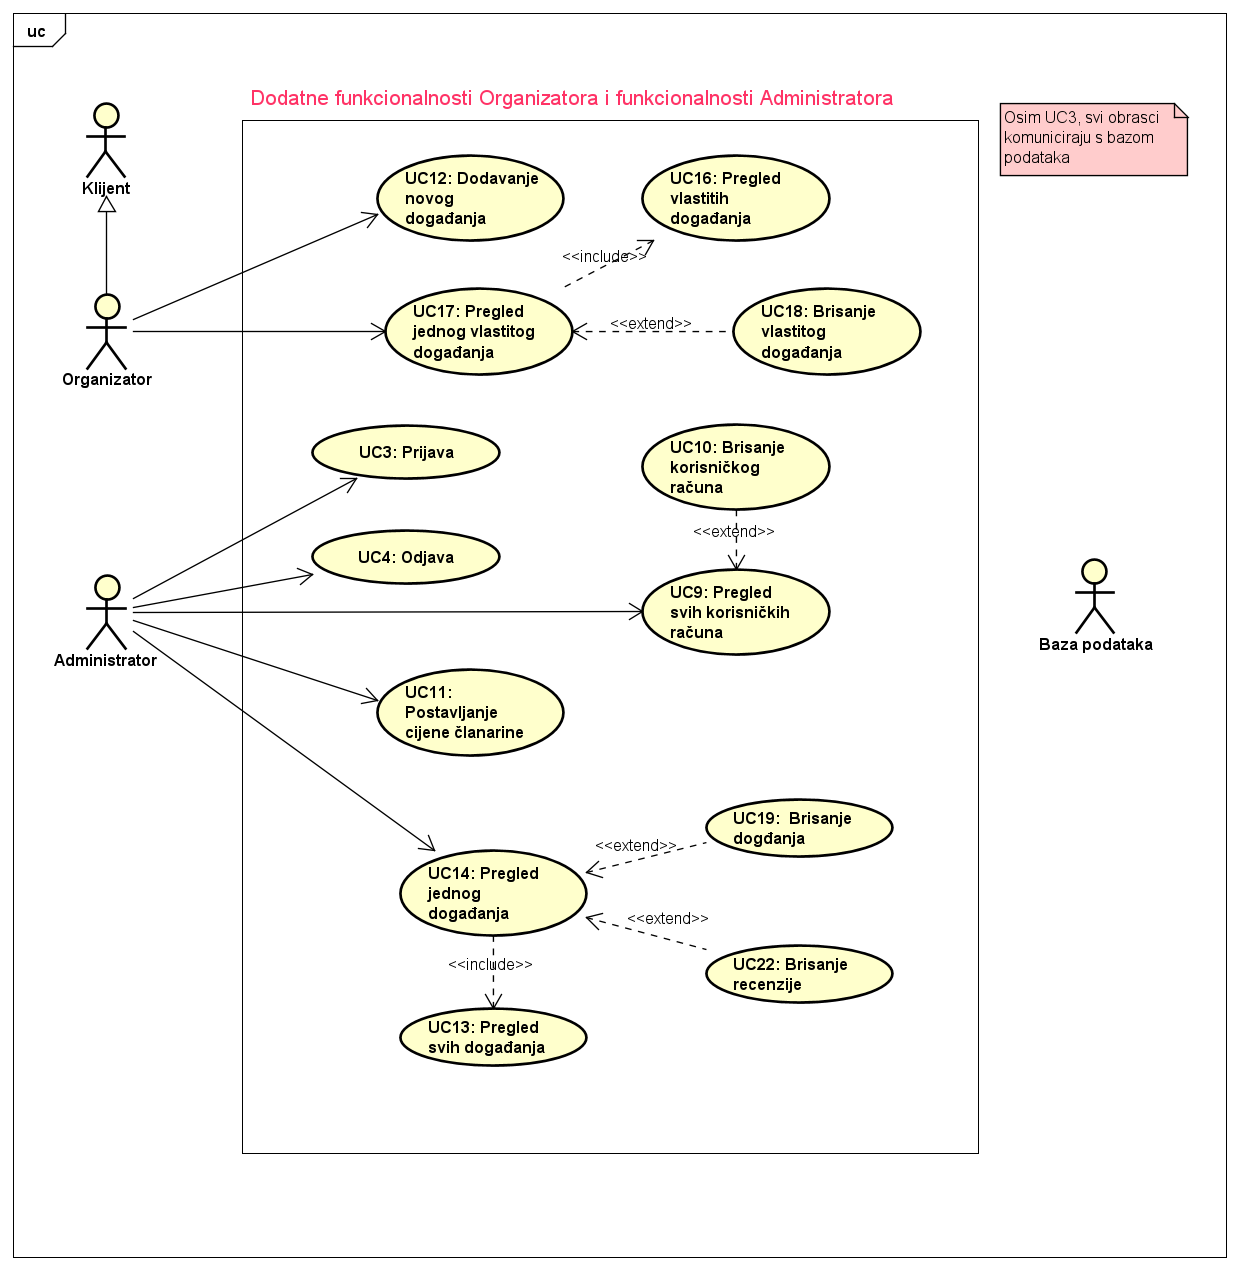
\includegraphics[scale=0.5]{dijagrami/uc2.PNG}
		\centering
		\caption{Dijagram obrazaca uporabe, dodatne funkcionalnosti Organizatora i funkcionalnost Administratora}
		\label{fig:promjene}
	\end{figure}
	
	\newpage
	
	\subsection{Sekvencijski dijagrami}
	
	\noindent \textbf{Obrazac upotrebe UC12 - Dodavanje novog događanja}
	
	\noindent Organizator odabire opciju dodavanja novog događanja. Prikazuje mu se obrazac za unos podataka o događanju. Po završetku unosa željenih podataka, organizator odabire opciju objave događanja. Provjeravaju se uneseni podaci - ako su ispravni, podaci o događanju spremaju se u bazu podataka i novo je događanje objavljeno, inače se prikazuje obavijest o neispravnosti podataka i organizatoru se omogućuje ponovni unos podataka o događanju. 
	
	\begin{figure}[H]
		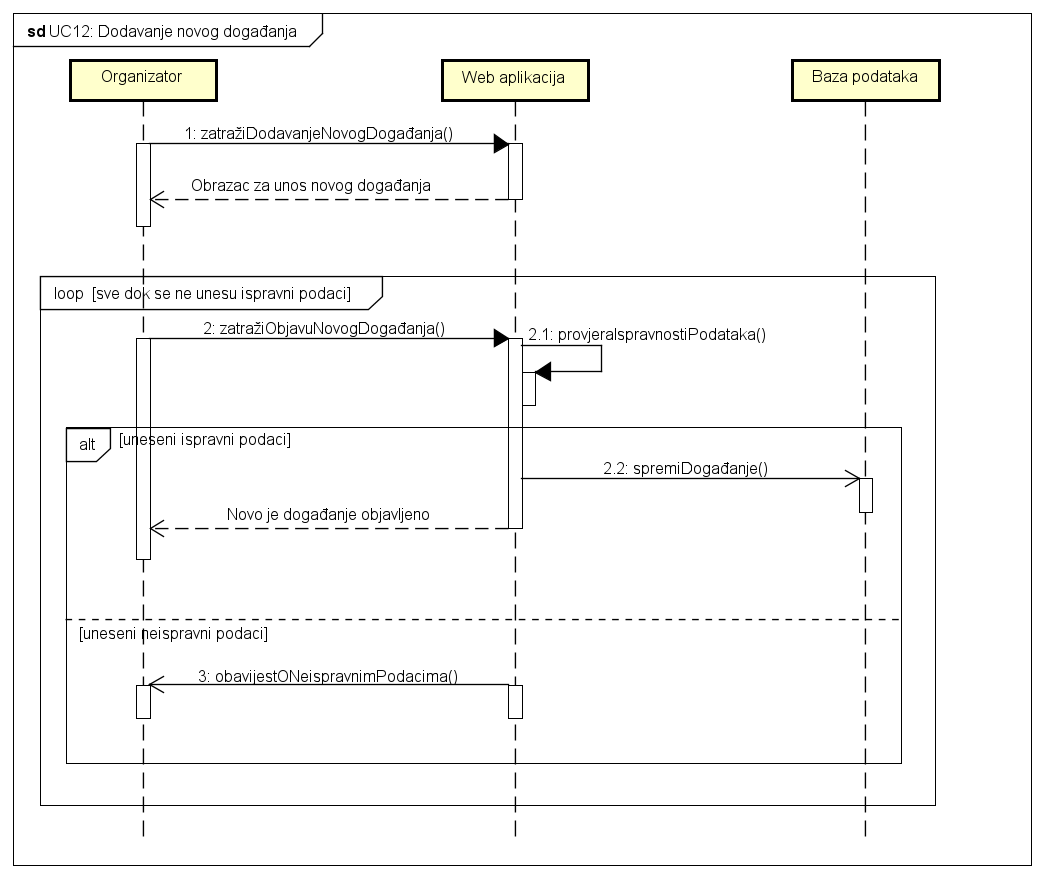
\includegraphics[width=\textwidth]{dijagrami/sd1.PNG}
		\centering
		\caption{Sekvencijski dijagram za \textbf{UC12}}
		\label{fig:promjene}
	\end{figure}
	
	\newpage
	
	\noindent \textbf{Obrazac upotrebe UC20 - Recenziranje događanja}
	
	\noindent Korisnik iz prikaza svih događanja završenih u posljednjih 48 sati odabire jedno koje želi recenzirati. Korisniku se vraća obrazac za unos recenzije. Pri objavi recenzije provjerava se ispravnost recenzije te ako je ispravna, recenzija se sprema u bazu podataka i prikazuje na stranici, u suprotnom korisnik se obavještava o neispravnosti recenzije i istu može napisati ponovno.
	
	\begin{figure}[H]
		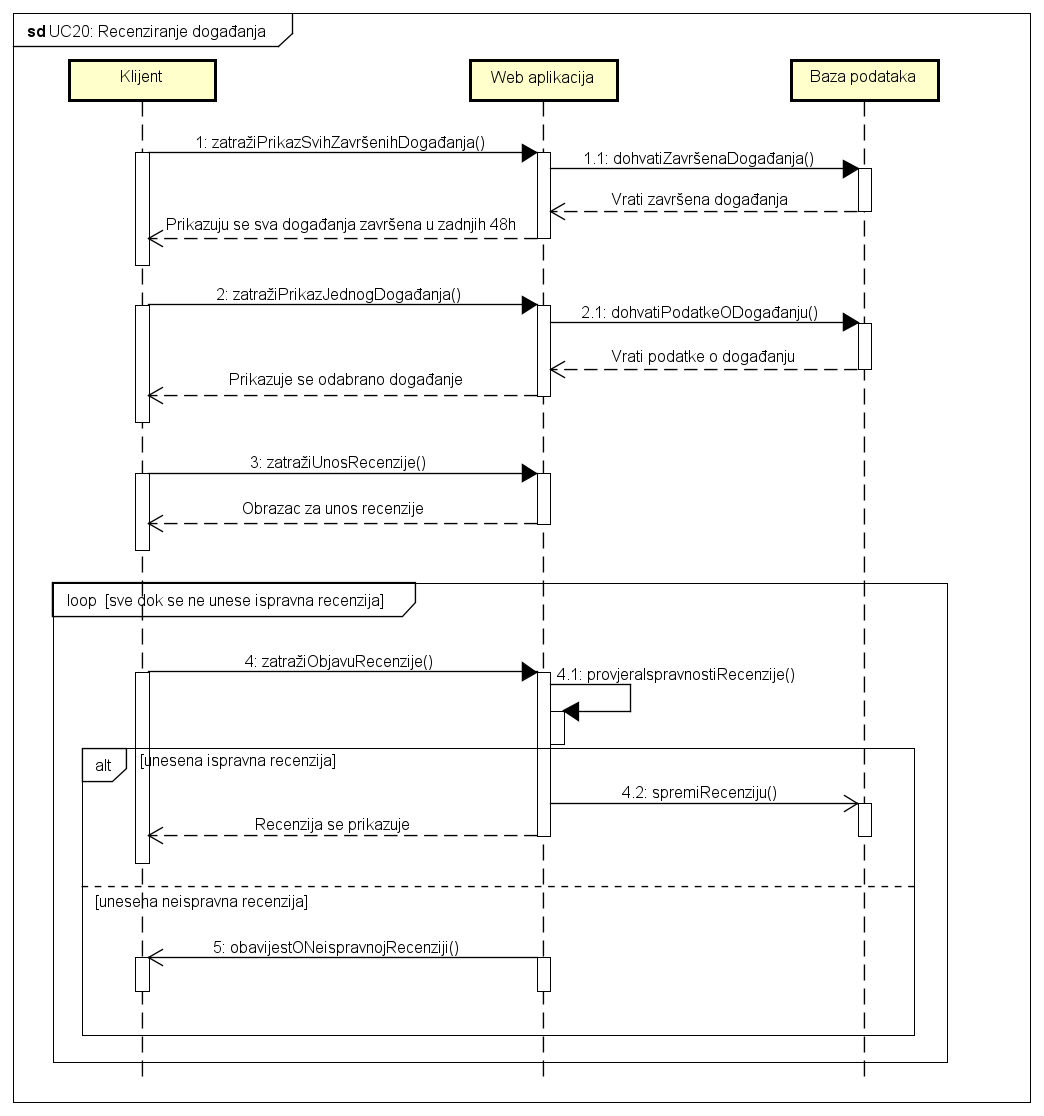
\includegraphics[width=\textwidth]{dijagrami/sd2.PNG}
		\centering
		\caption{Sekvencijski dijagram za \textbf{UC20}}
		\label{fig:promjene}
	\end{figure}
	
	\newpage
	
	\noindent \textbf{Obrazac upotrebe UC23 - Iskazivanje interesa za događanje}
	
	\noindent Korisnik iz prikaza svih događanja završenih u posljednjih odabire jedno za koje želi iskazati interes. Korisniku odabire jednu od opcija \textit{sigurno dolazim}, \textit{možda dolazim}, \textit{ne dolazim}. Obavlja se provjera baze podataka i utvrđuje je li to prvi iskazani interes tog korisnika za događanje ili se radi o promjeni iskazanog interesa. U bazu se sprema novi zapis ili se postojeći mijenja i na stranici korisnik vidi svoj iskazan interes.
	
	\begin{figure}[H]
		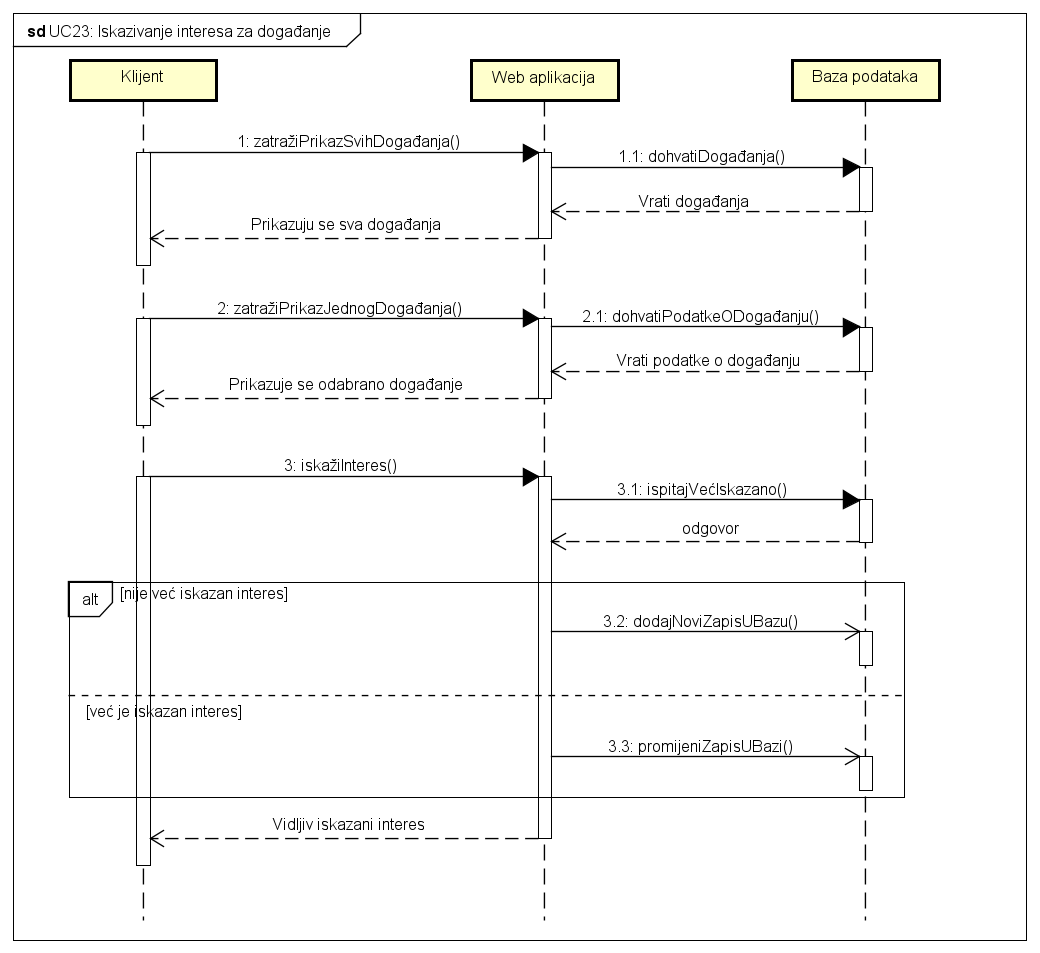
\includegraphics[width=\textwidth]{dijagrami/sd3.PNG}
		\centering
		\caption{Sekvencijski dijagram za \textbf{UC23}}
		\label{fig:promjene}
	\end{figure}
	
	\newpage
	
	\noindent \textbf{Obrasci upotrebe UC9, UC10 i UC11 - Prikaz i brisanje korisničkih računa i postavljanje cijene članarine}
	
	\noindent Administrator odabire opciju prikaza svih korisničkih računa koji se po tom odabiru dohvaćaju iz baze. Kraj korisničkog računa na popisu, administrator može odabrati opciju brisanja korisničkog računa te se brisanje obavlja nakon potvrde. Odabirom opcije za promjenu iznosa članarine administratoru se vraća obrazac u koji administrator unosi novu cijenu članarine sve dok ne unese ispravan iznos.
	
	\vspace{-0.4cm}
	
	\begin{figure}[H]
		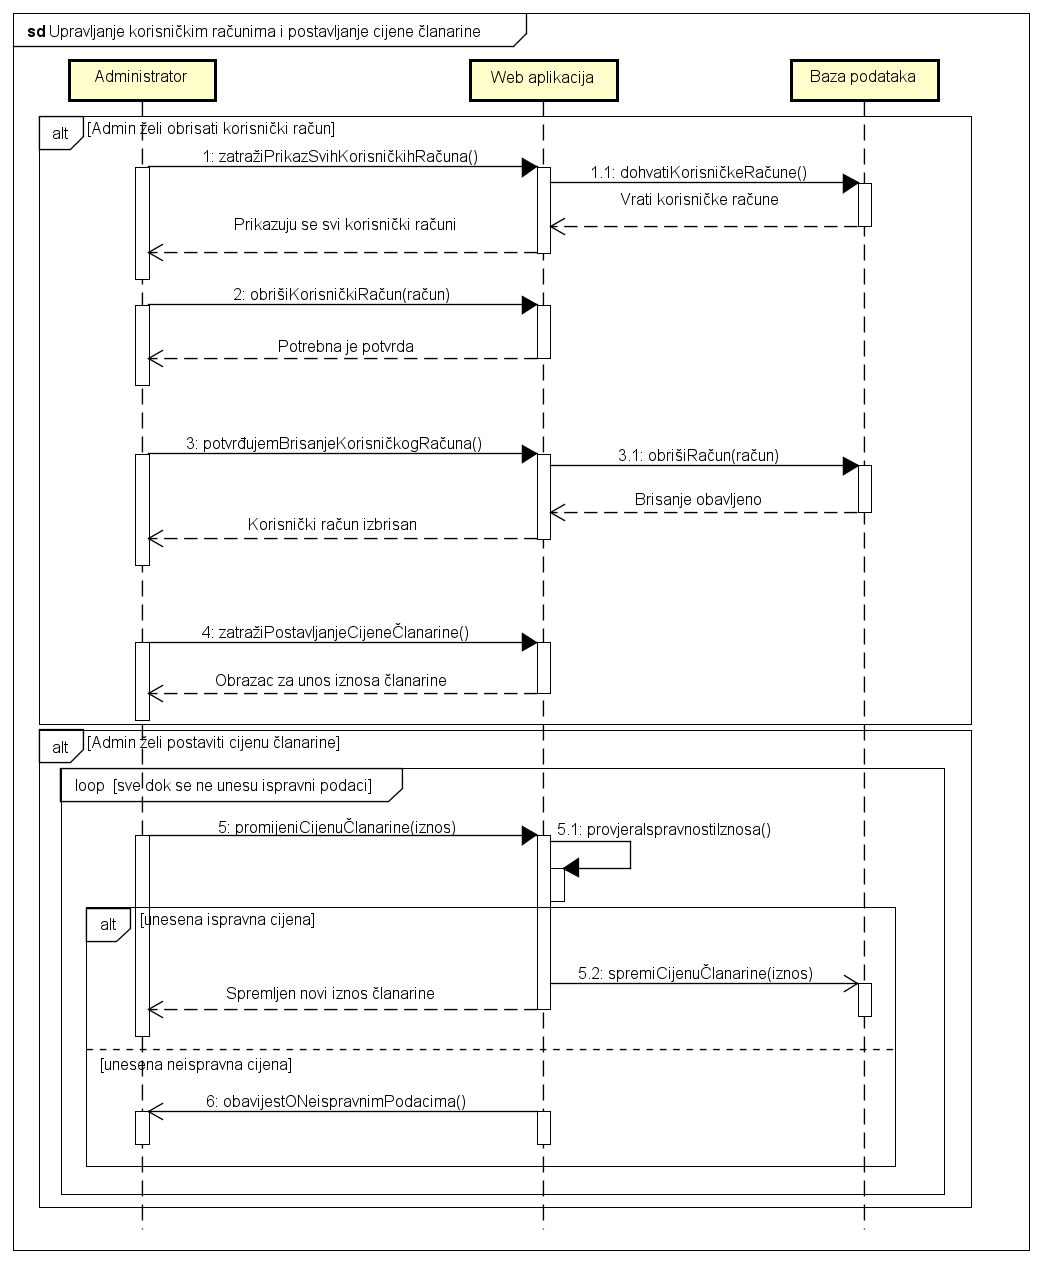
\includegraphics[width=\textwidth]{dijagrami/sd4.PNG}
		\centering
		\vspace{-1cm}
		\caption{Sekvencijski dijagram za \textbf{UC9}, \textbf{UC10} i \textbf{UC11}}
		\label{fig:promjene}
	\end{figure}
	
	\vspace{-0.6cm}
	
	\newpage
	
	\section{Ostali zahtjevi}
	
	\begin{packed_item}
		\item Sustav treba biti implementiran kao web aplikacija koristeći objektno-orijentirane jezike 
		\item Sustav mora omogućiti rad više korisnika u stvarnom vremenu 
		\item Sustav treba sve zadatke izvršavati u vrlo kratkom vremenu, unutar nekoliko sekundi
		\item Korisnički podaci trebaju biti sigurno pohranjeni i odgovarajuće enkriptirani
		\item Sustav mora efikasno pohranjivati, upravljati i pristupati podacima putem baze podataka 
		\item Korisničko sučelje mora podržavati hrvatsku abecedu pri unosu i prikazu tekstualnog sadržaja
		\item Sustav mora koristiti europsku valutu (EUR) za prikaz cijena te europski oblik datuma (\textit{DD.MM.GGGG}) za prikaz i unos datuma
		\item Web aplikacija mora biti responzivna i optimalno korisničko iskustvo pružati na svim uređajima
		\item Korisničko sučelje treba biti intuitivno i pregledno, korisnici se moraju moći koristiti sučeljem bez opširnih uputa
		\item Neispravno korištenje korisničkog sučelja ne smije narušiti funkcionalnosti i rad sustava
		
		
	\end{packed_item}
	
	

	\chapter{Arhitektura i dizajn sustava}

		
	%	\textbf{\textit{dio 1. revizije}}\\

%		\textit{ Potrebno je opisati stil arhitekture te identificirati: podsustave, preslikavanje na radnu platformu, spremišta podataka, mrežne protokole, globalni upravljački tok i sklopovsko-programske zahtjeve. Po točkama razraditi i popratiti odgovarajućim skicama:}
%	\begin{itemize}
%		\item 	\textit{izbor arhitekture temeljem principa oblikovanja pokazanih na predavanjima (objasniti zašto ste baš odabrali takvu arhitekturu)}
%		\item 	\textit{organizaciju sustava s najviše razine apstrakcije (npr. klijent-poslužitelj, baza podataka, datotečni sustav, grafičko sučelje)}
%		\item 	\textit{organizaciju aplikacije (npr. slojevi frontend i backend, MVC arhitektura) }		
%	\end{itemize}

		\noindent Arhitektura sustava sastoji se od tri glavna dijela: 
		
		\begin{packed_item}
			\item Web preglednik 
			\item Web poslužitelj
			\item Baza podataka
		\end{packed_item}
		
		\textbf{Web preglednik} računalni je program koji korisnicima omogućuje  pristup internetu i pregled web stranica te interakciju s raznim online sadržajem. Korisnici koriste web preglednik za slanje zahtjeva web poslužitelju putem HTTP (eng. \textit{Hyper Text Transfer Protocol}) protokola i primanje odgovora u obliku HTML dokumenata koji se zatim interpretiraju i prikazuju. Osim pregledavanja web stranica, web preglednici omogućuju i izvođenje različitih aktivnosti kao što su ispunjavanje web obrazaca i prikaz slika i videozapisa.
		
		\textbf{Web poslužitelj} ključan je dio web aplikacija i internetskih servisa. Njegova je glavna uloga primanje, obrada i posredovanje zahtjeva koji dolaze od web preglednika korisnika. Web poslužitelj uspostavlja komunikaciju između klijenta (korisnika) i web aplikacije te osigurava ispravan protok informacija.
		
		\textbf{Web aplikacija} obrađuje zahtjeve korisnika. Nakon obrade zahtjeva, šalje se odgovor poslužitelju koji se korisniku prikazuje u web pregledniku. Obrada korisničkih zahtjeva najčešće uključuje određenu komunikaciju s bazom podataka npr. dohvaćanje, uređivanje ili brisanje podataka. \\
		
				
		Aplikacija je izgrađena korištenjem objektno orijentirane paradigme. Za poslužiteljski dio (\textit{backend}) korišten je radni okvir Java Spring Boot. Za izradu korisničkog sučelja (\textit{frontend}) koristi se open-source JavaScript biblioteka React. Odabrana su razvojna okruženja Visual Studio Code i IntelliJ IDEA.\\
		 
		 
		\noindent Korišteni Spring razvojni okvir koristi se MVC arhitekturom (eng. \textit{Model-View-Controller}). MVC arhitekturni obrazac razdvaja prezentaciju podataka, dohvat i manipulaciju podataka. MVC obuhvaća sljedeću podjelu uloga prikazanu i na slici \ref{arh}:
		
		\begin{packed_item}
			\item \textbf{Model} - sadrži razrede čiji objekti se obrađuju; služi za dohvat i manipulaciju podacima
			\item \textbf{View} - sadrži razrede čiji objekti služe za prikaz podataka; odlučuje kako će se dohvaćeni podaci prikazati
			\item \textbf{Controller} - prima zahtjeve za resursima od klijenta koje
			obrađuje i prosljeđuje; upravlja ostalim elementima sustava
		\end{packed_item}
		
		
		\begin{figure}[H]
			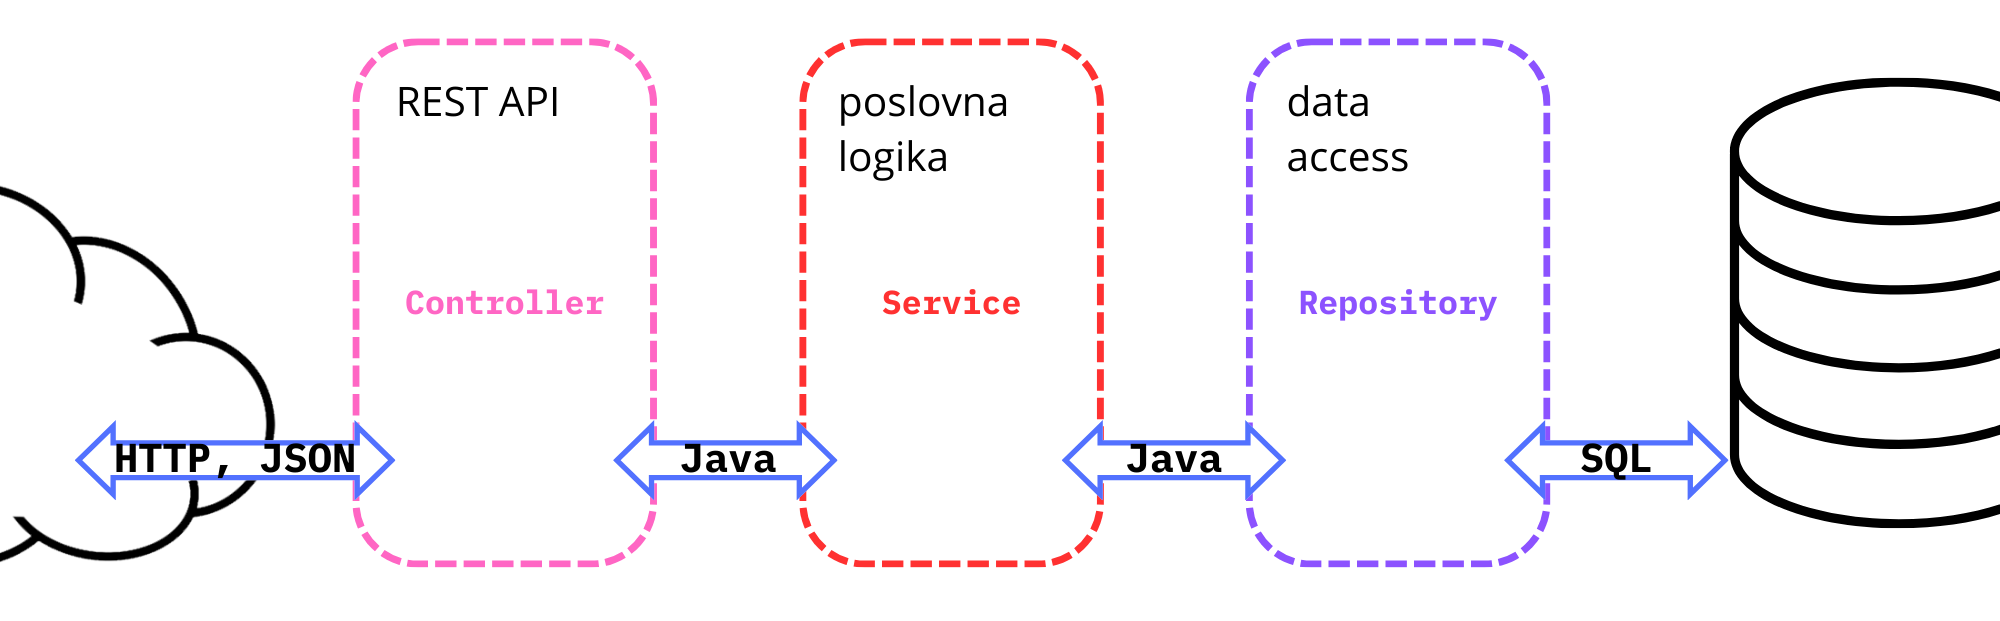
\includegraphics[width=\textwidth]{slike/mvc-arh.PNG}
			\centering
			\caption{Prikaz MVC arhitekture}
			\label{arh}
		\end{figure}
		
		\newpage
		
		\section{Baza podataka}
			
		Sustav koristi H2 relacijsku bazu podataka za organizaciju i pohranu različitih podataka. Organizacija temeljena na relacijskom modelu omogućuje lakšu manipulaciju podacima, pruža sigurnost i kontrolu nad podacima te osigurava trajno spremanje podataka. U sustavu baza podataka igra ključnu ulogu u pohrani informacija o korisnicima, događanjima i dodatnim informacijama o događanjima. Baza podataka ima sljedeće entitete:
		
		\begin{packed_item}
			\item Korisnik
			\item Dogadjanje
			\item Poveznica
			\item MedijskiSadrzaj
			\item Recenzija
			\item DolazakKorisnika
			\item Clanarina
			\item Pretplata
		\end{packed_item}
		
		\noindent Svaki od entiteta ima svoje atribute i jedinstveni primarni ključ koji osigurava jednoznačno identificiranje svakog zapisa. Baza podataka omogućuje brzu i jednostavnu pohranu, izmjenu i dohvat podataka, što je ključno za daljnju obradu podataka o događanjima.
		
			\subsection{Opis tablica}
			
				\noindent \textbf{Korisnik} Entitet sadrži sve relevantne informacije o registriranom korisniku aplikacije. Atributi id, korisnickoime, email, lozinka i tipkorisnika spremaju se za sve tipove korisnika sustava, dok se atributi adresa i placanjeclanarine odnose samo na organizatore i poprimaju vrijednost \textit{null} za tip korisnika Posjetitelj i Administrator.
				
				\begin{longtblr}[
					label=none,
					entry=none
					]{
						width = \textwidth,
						colspec={|X[8,l]|X[6, l]|X[20, l]|}, 
						rowhead = 1,
					}
					\hline \SetCell[c=3]{c}{\textbf{Korisnik}}	 \\ \hline[3pt]
					\SetCell{LightGreen}
					id & BIGINT	&  	jedinstveni identifikator korisnika  	\\ 
					\hline
					korisnickoime	& VARCHAR & korisničko ime\\ 
					\hline 
					email & VARCHAR & e-mail adresa korisnika  \\
					 \hline 
					lozinka & VARCHAR	&  lozinka korisničkog računa \\ 
					\hline 
					tipkorisnika & VARCHAR	& Posjetitelj, Organizator ili Administrator\\ 
					\hline 
					adresa & VARCHAR & adresa Organizatora\\ 
					\hline 
					placanjeclanarine & BOOLEAN	& plaća li Organizator članarinu\\ 
					\hline
				\end{longtblr}
				
				\noindent \textbf{Dogadjanje} Entitet omogućuje pohranu informacija o različitim događanjima koja se mogu organizirati. Atribut organizatorid strani je ključ koji se odnosi na korisnika koji je organizator događanja. Atribut cijenaulaznice sadrži informacije o cijeni ulaznica za događanje, a može biti i \textit{null} u slučaju da je događanje besplatno. 
				
				\begin{longtblr}[
					label=none,
					entry=none
					]{
						width = \textwidth,
						colspec={|X[8,l]|X[6, l]|X[20, l]|}, 
						rowhead = 1,
					} 
					\hline \SetCell[c=3]{c}{\textbf{Dogadjanje}}	 \\ \hline[3pt]
					\SetCell{LightGreen}
					iddogadjanja & BIGINT	&  	jedinstveni identifikator događanja  	\\ 
					\hline
					nazivdogadjanja	& VARCHAR & naziv događanja \\ 
					\hline 
					tipdogadjanja & VARCHAR & vrsta događanja  \\
					\hline 
					lokacijagodadjanja & VARCHAR & lokacija događanja \\ 
					\hline 
					vrijemedogadjanja & TIMESTAMP & datum i vrijeme događanja\\ 
					\hline 
					trajanje & DOUBLE & vremensko trajanje događanja\\ 
					\hline 
					\SetCell{LightBlue} organizatorid & BIGINT	& identifikator Organizatora \\ 
					\hline
					cijenaulaznice & DOUBLE	& cijena ulaznice događanja\\ 
					\hline
				\end{longtblr}
				
				\noindent \textbf{Poveznica} Entitet služi za pohranu podataka o poveznicama koje su povezane s određenim organizatorima događanja (strani ključ organizatorid). 
				
				\begin{longtblr}[
					label=none,
					entry=none
					]{
						width = \textwidth,
						colspec={|X[8,l]|X[6, l]|X[20, l]|}, 
						rowhead = 1,
					} 
					\hline \SetCell[c=3]{c}{\textbf{Poveznica}}	 \\ \hline[3pt]
					\SetCell{LightGreen}
					idpoveznice & BIGINT & jedinstveni identifikator poveznice  	\\ 
					\hline
					\SetCell{LightBlue} organizatorid & BIGINT	& identifikator Organizatora \\ 
					\hline
					link & VARCHAR	& poveznica na web stranice Organizatora\\ 
					\hline
				\end{longtblr}
				
				\noindent \textbf{MedijskiSadrzaj} Entitet omogućava pohranu različitih medijskih sadržaja koji su povezani s određenim događanjima, što omogućava organizatorima da dijele fotografije i videozapise povezane s njihovim događanjima.
				
				\begin{longtblr}[
					label=none,
					entry=none
					]{
						width = \textwidth,
						colspec={|X[10,l]|X[6, l]|X[20, l]|}, 
						rowhead = 1,
					} 
					\hline \SetCell[c=3]{c}{\textbf{MedijskiSadrzaj}}	 \\ \hline[3pt]
					\SetCell{LightGreen}
					idmedijskogsadrzaja & BIGINT & jedinstveni identifikator sadržaja  	\\ 
					\hline
					\SetCell{LightBlue} iddogadjanja & BIGINT	& identifikator događanja \\ 
					\hline
					medijskisadrzaj & LONGLOB & medijski sadržaj\\ 
					\hline
				\end{longtblr}
				
				\noindent \textbf{Recenzija} Entitet služi za pohranu recenzija koje korisnici mogu napisati za određena događanja u sustavu. Entitet omogućava korisnicima da izraze svoje mišljenje i ocjene događanja, čime se pruža povratna informacija organizatorima i drugim potencijalnim sudionicima.
				
				
				\begin{longtblr}[
					label=none,
					entry=none
					]{
						width = \textwidth,
						colspec={|X[8,l]|X[6, l]|X[20, l]|}, 
						rowhead = 1,
					} 
					\hline \SetCell[c=3]{c}{\textbf{Recenzija}}	 \\ \hline[3pt]
					\SetCell{LightGreen}
					idrecenzije & BIGINT	&  	jedinstveni identifikator recenzije\\ 
					\hline
					recenzijatekst & TEXT & tekst napisane  recenzije \\
					\hline
					ocjena & INT & dodijeljena ocjena događanja\\
					\hline 
					\SetCell{LightBlue} iddogadjanja & BIGINT & identifikator događanja\\
					\hline 
					\SetCell{LightBlue} idkorisnik & BIGINT & identifikator korisnika (autora recenzije)\\ 
					\hline
				\end{longtblr}
				
				\noindent \textbf{DolazakKorisnika} Entitet služi za praćenje iskazanog interesa korisnika za dolazak na određeno događanje. Atribut statusdolaska može poprimiti vrijednosti \textit{sigurno dolazim}, \textit{možda dolazim} i \textit{ne dolazim}.
				
				\begin{longtblr}[
					label=none,
					entry=none
					]{
						width = \textwidth,
						colspec={|X[9,l]|X[6, l]|X[20, l]|}, 
						rowhead = 1,
					} 
					\hline \SetCell[c=3]{c}{\textbf{DolazakKorisnika}}	 \\ \hline[3pt]
					\SetCell{LightGreen}
					iddolaskakorisnika & BIGINT	&  	jedinstveni identifikator dolaska  	\\ 
					\hline
					statusdolaska & VARCHAR & iskazani interes za dolazak \\ 
					\hline 
					\SetCell{LightBlue} iddogadjanja & BIGINT & identifikator događanja  \\
					\hline 
					\SetCell{LightBlue} idkorisnik & BIGINT & identifikator korisnika\\ 
					\hline
				\end{longtblr}
				
				\noindent \textbf{Clanarina} Entitet služi za praćenje informacija o članarinama koje organizatori moraju platiti kako bi imali mogućnost organiziranja događanja za koja se plaća ulaz. Entitet omogućava praćenje članarina koje su korisnici platili te pruža informacije o cijenama i datumima isteka vrijednosti članarine.
				
				\begin{longtblr}[
					label=none,
					entry=none
					]{
						width = \textwidth,
						colspec={|X[8,l]|X[6, l]|X[20, l]|}, 
						rowhead = 1,
					} 
					\hline \SetCell[c=3]{c}{\textbf{Clanarina}}	 \\ \hline[3pt]
					\SetCell{LightGreen}
					idclanarine & BIGINT	&  	jedinstveni identifikator članarine \\ 
					\hline
					\SetCell{LightBlue} idkorisnik & BIGINT & identifikator korisnika \\ 
					\hline 
					cijenaclanarine & DOUBLE & iznos cijene članarine  \\
					\hline 
					vrijedido & TIMESTAMP & datum i vrijeme isteka članarine\\ 
					\hline
				\end{longtblr}
				
				\noindent \textbf{Pretplata} Entitet služi za spremanje korisničkih postavki o automatskom slanju obavijesti o novim događanjima. Posjetitelji mogu odabrati postavke da im aplikacija automatski šalje obavijesti o najnovijim događanjima prema kriterijima vrsta (kategorija) događanja i područje (lokacija).  
				
				\begin{longtblr}[
					label=none,
					entry=none
					]{
						width = \textwidth,
						colspec={|X[8,l]|X[6, l]|X[20, l]|}, 
						rowhead = 1,
					} 
					\hline \SetCell[c=3]{c}{\textbf{Pretplata}}	 \\ \hline[3pt]
					\SetCell{LightGreen}
					idpretplata & BIGINT &  jedinstveni identifikator pretplate \\
					\hline 
					\SetCell{LightBlue} idkorisnik & BIGINT & identifikator korisnika \\ 
					\hline 
					kategorija & VARCHAR & kategorija za koju želi primati obavijesti\\
					\hline 
					lokacija & VARCHAR & lokacija za koju želi primati obavijesti\\ 
					\hline
				\end{longtblr}
				
				\newpage
				
			
			\subsection{Dijagram baze podataka}
				
				\begin{figure}[H]
					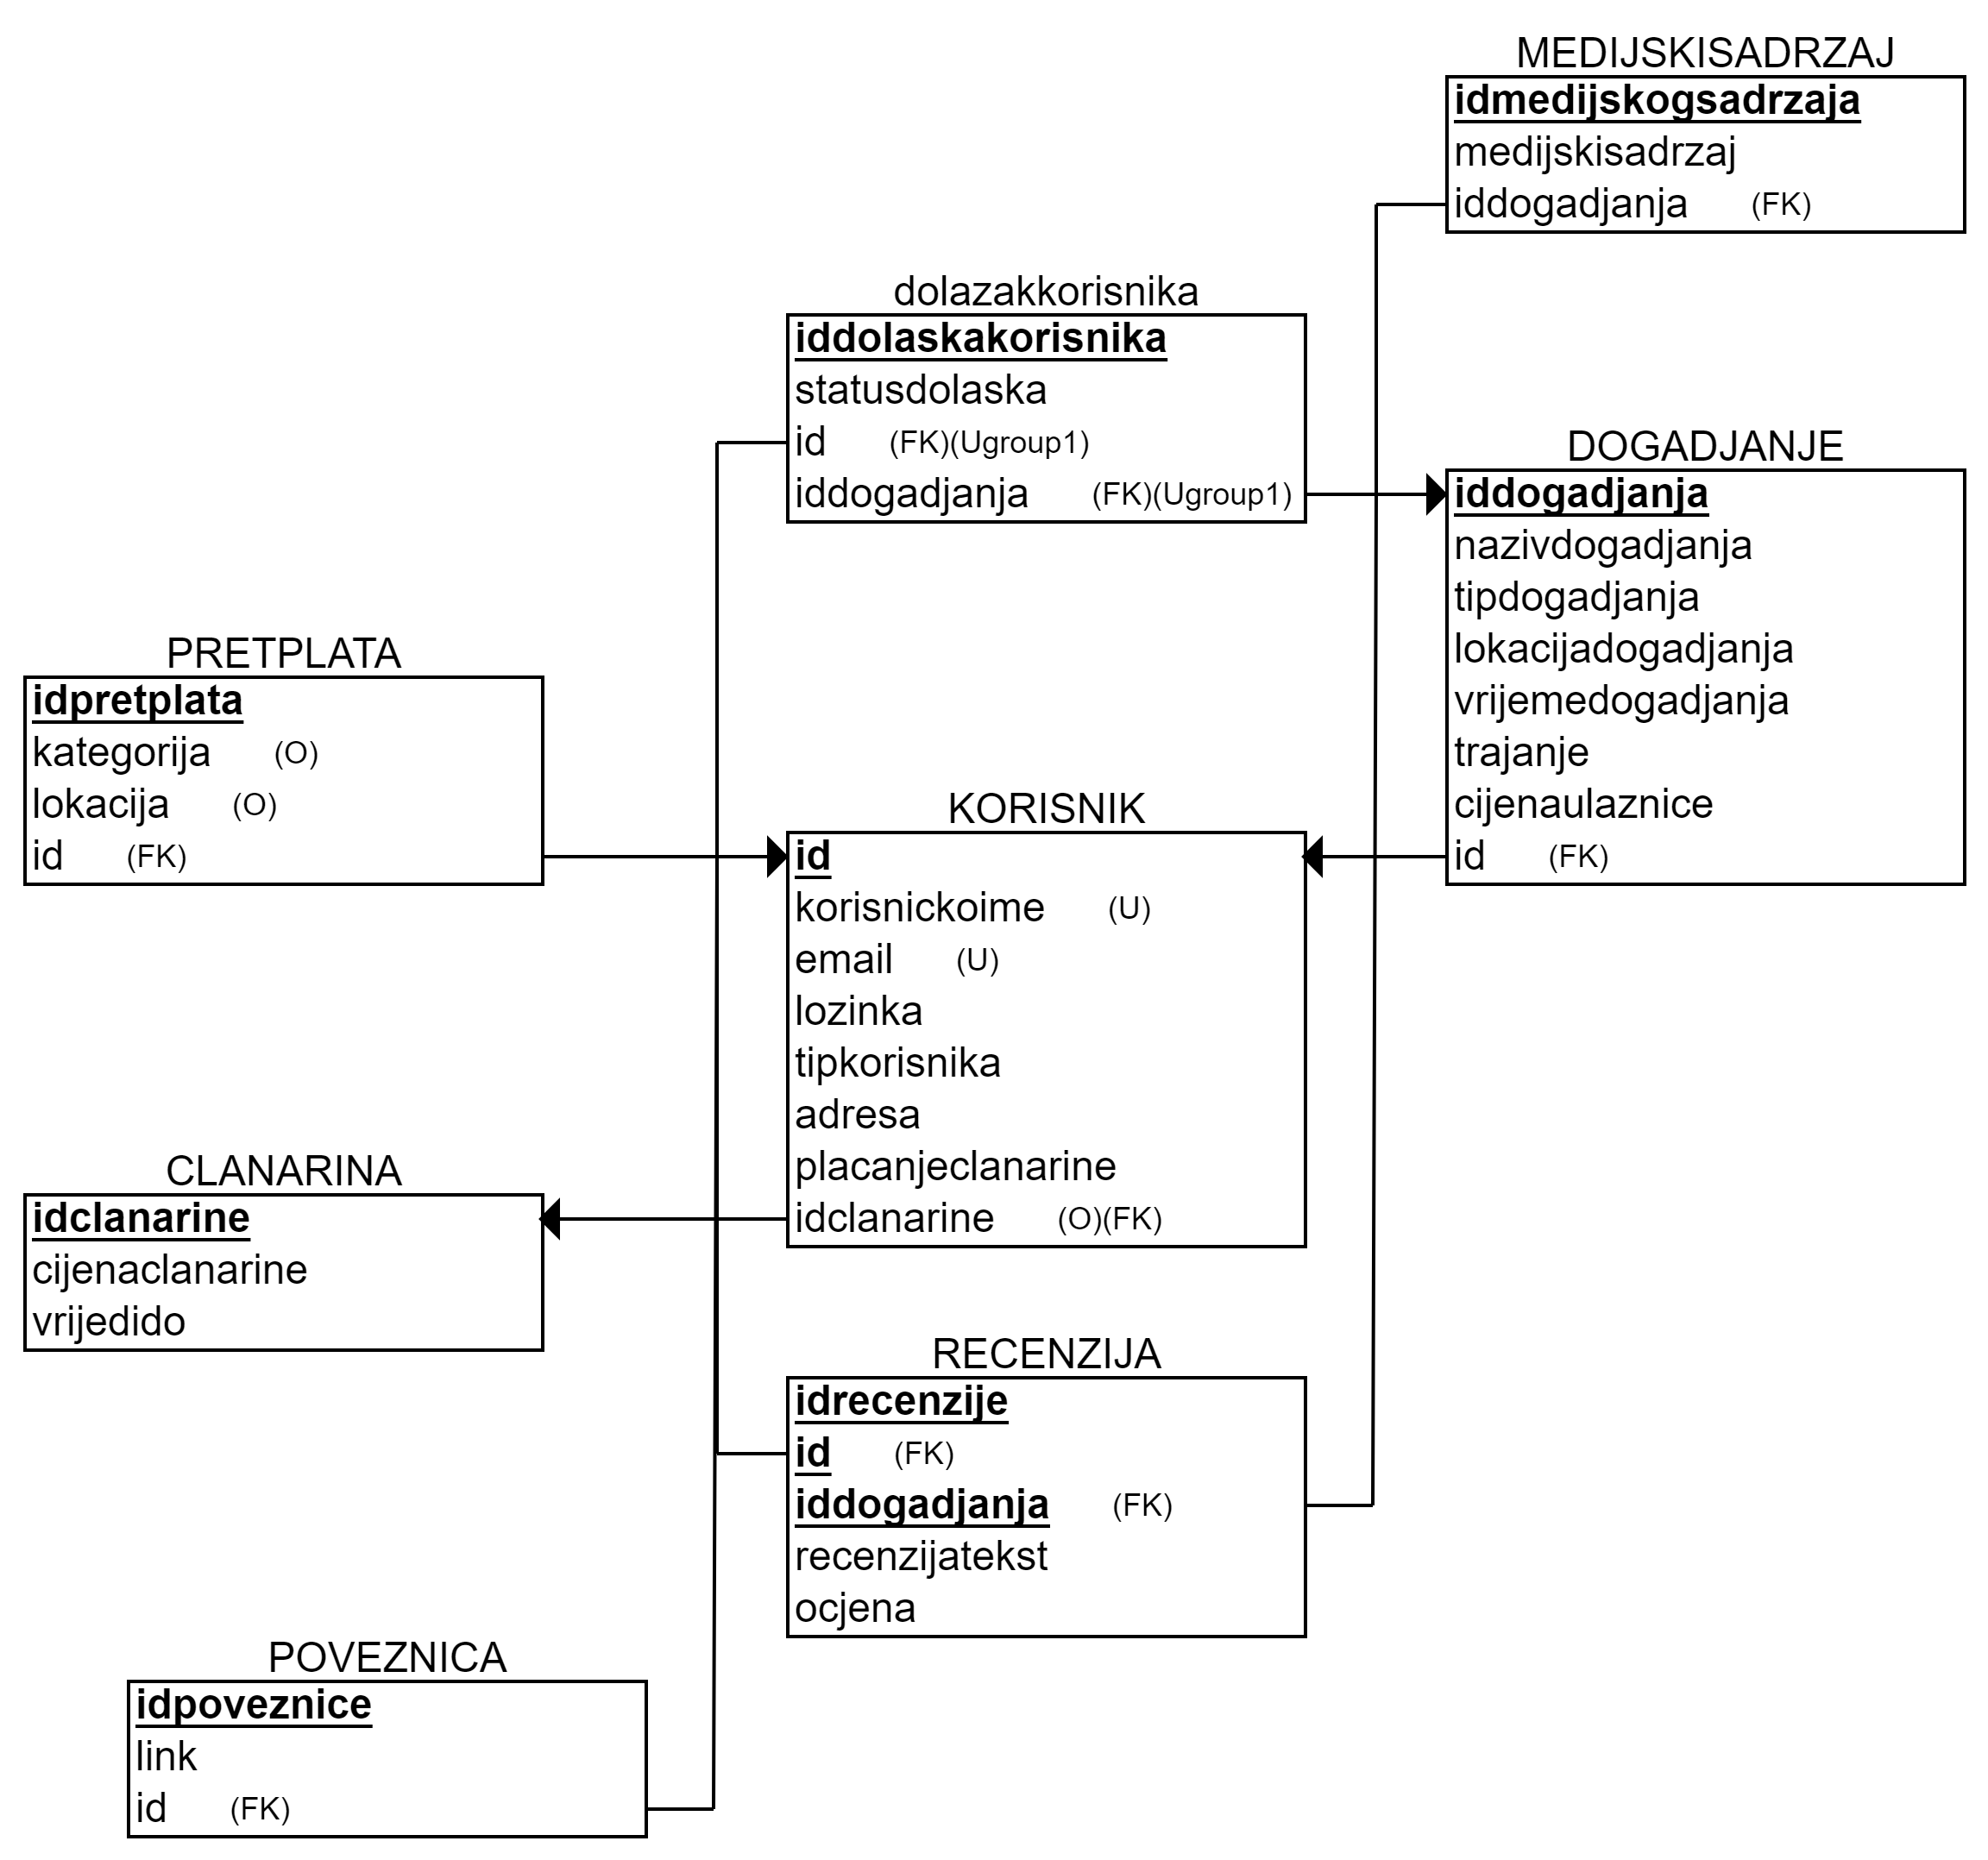
\includegraphics[width=\textwidth]{dijagrami/db_REL.png} 
					\centering
					\caption{Dijagram baze podataka}
					\label{fig:promjene}
				\end{figure}
				
				\newpage
				
				\begin{figure}[H]
					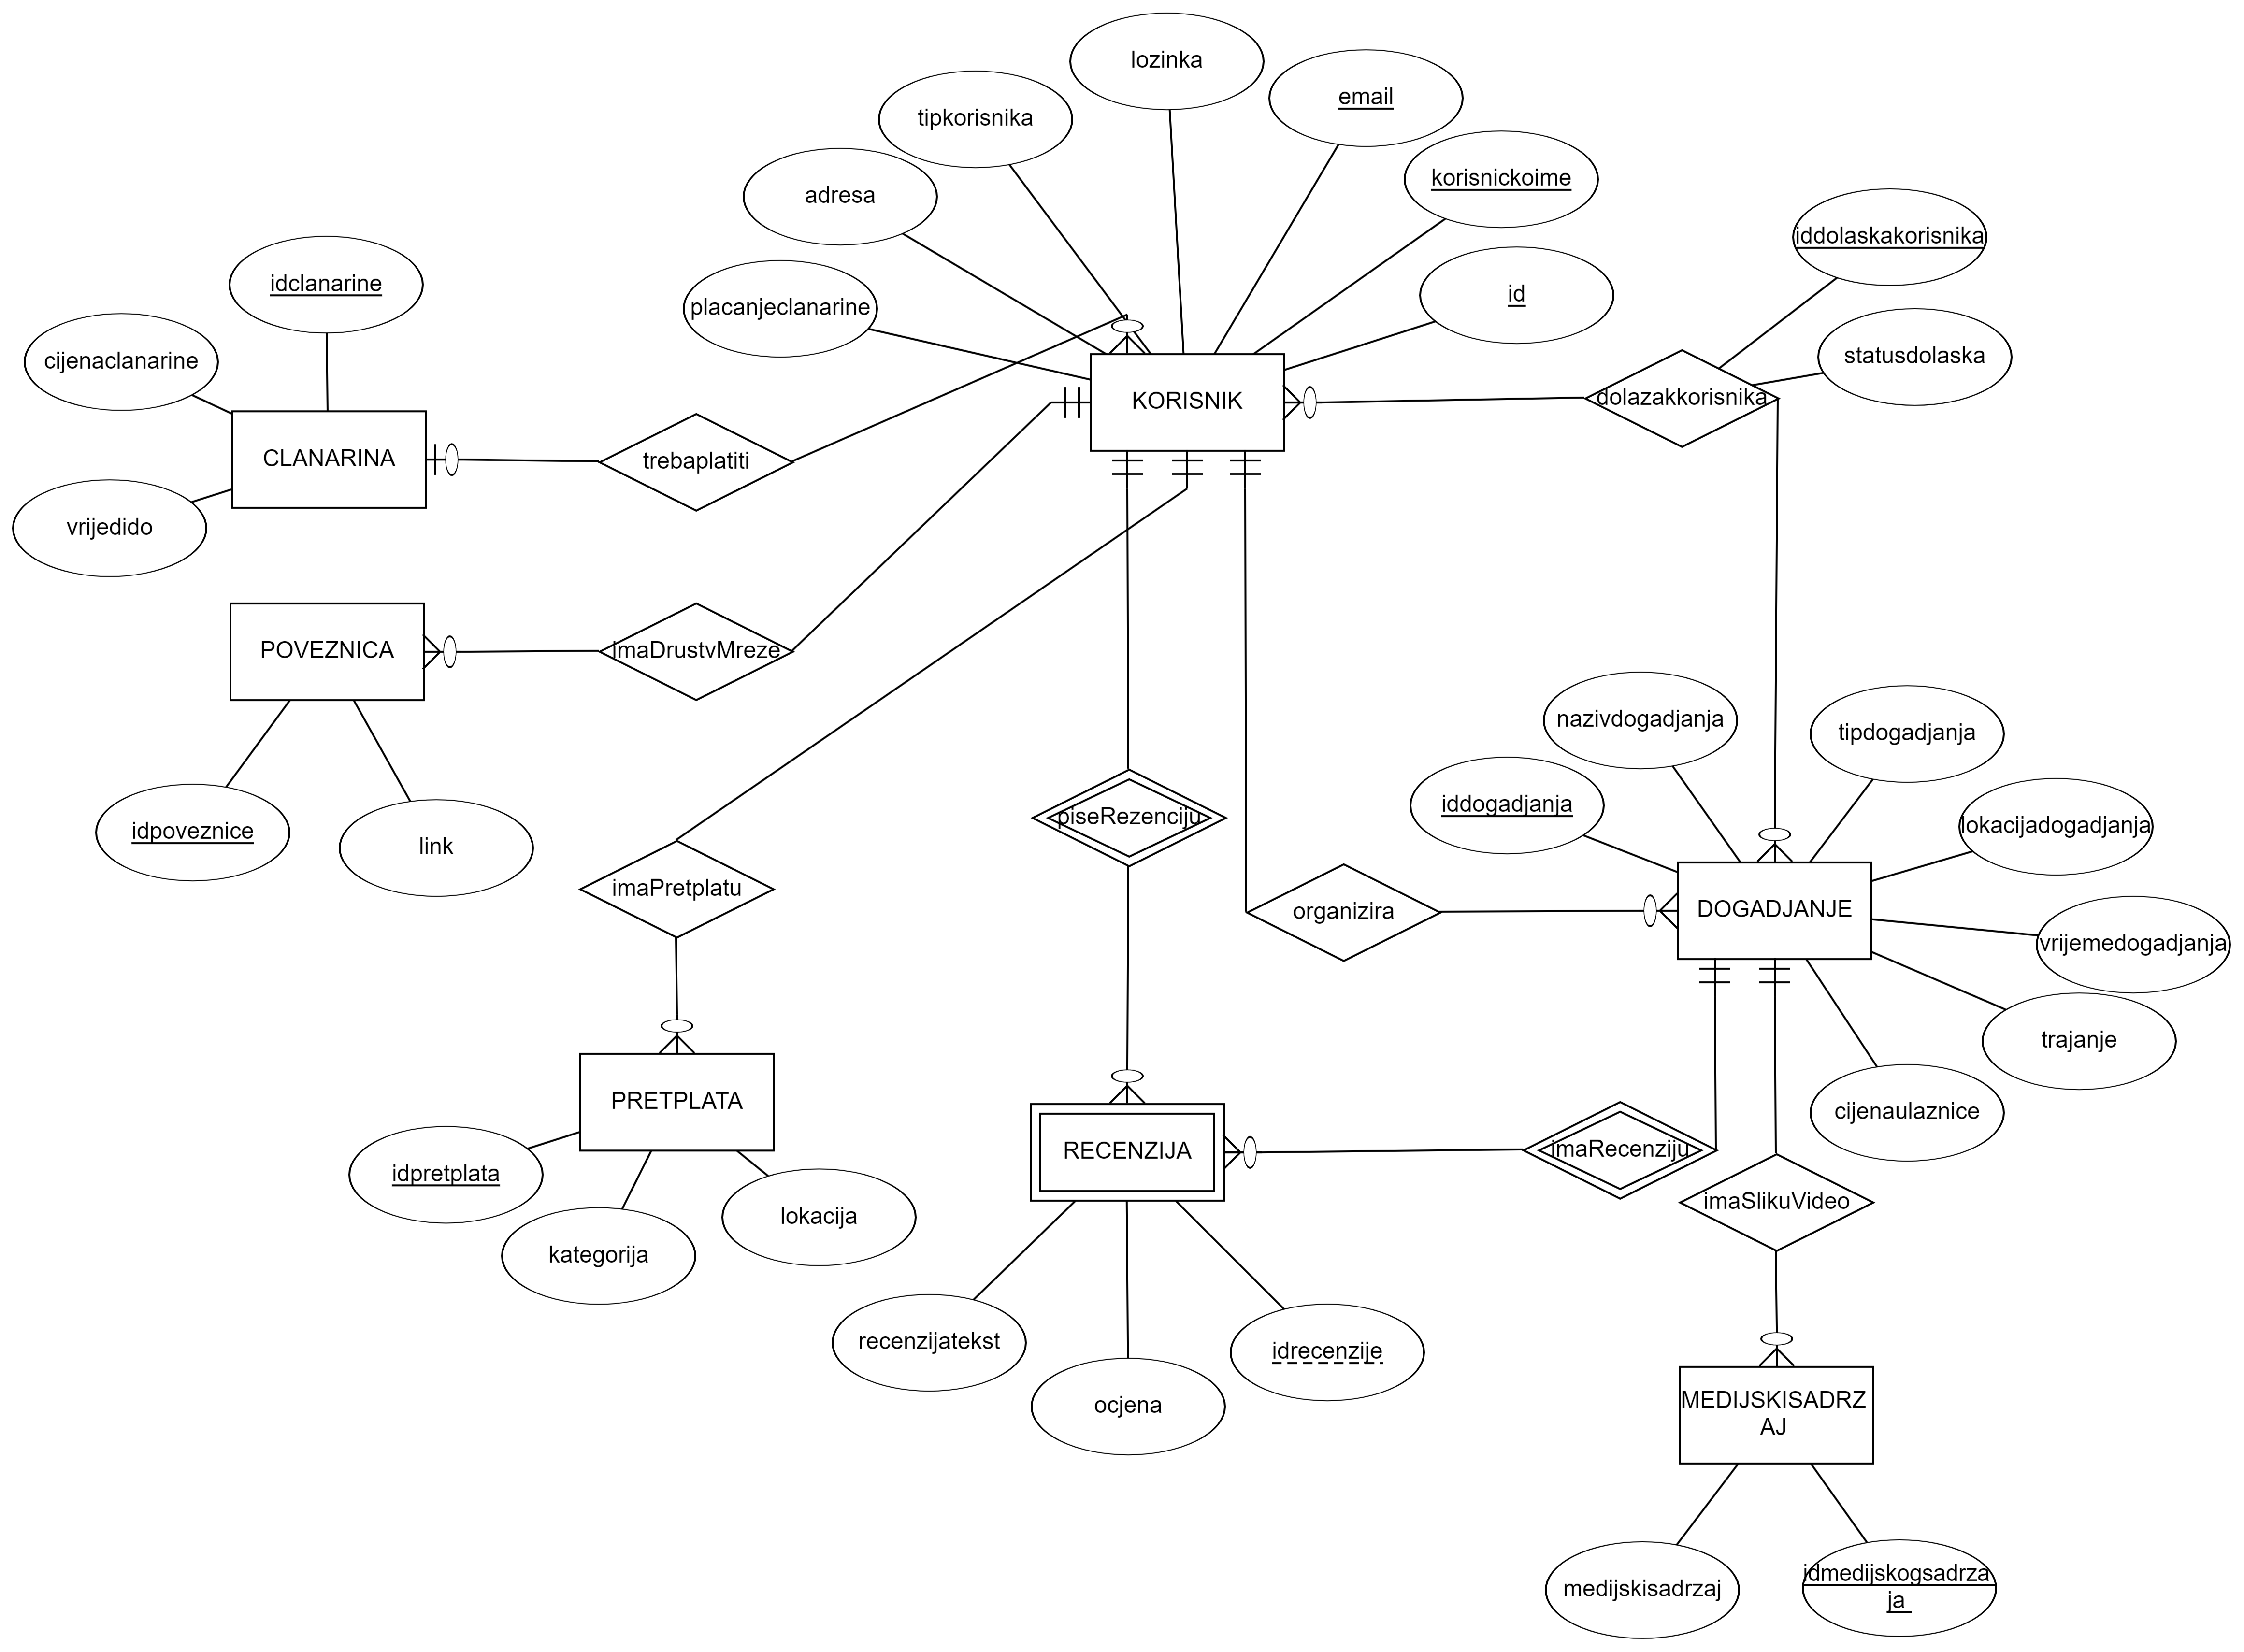
\includegraphics[width=\textwidth]{dijagrami/db_ER.png} 
					\centering
					\caption{ER dijagram baze podataka}
				\end{figure}
				
			\eject
			
			
		\section{Dijagram razreda}
		
		Dijagrami razreda prikazuju razrede u objektno orijentiranom sustavu, njihove atribute i
		metode te veze između razreda koji međusobno komuniciraju ili se nasljeđuju. Na slikama su prikazani razredi koji odgovaraju backend dijelu MVC arhitekture. Slika \ref{cd2} prikazuje sučelja koja pripadaju sloju Repository. Razredi prikazani na slici \ref{cd3} nasljeđuju Controller razred. Na slici \ref{cd5} prikazan je sloj Services, a na slici \ref{cd4} Data transfer objects. Razredi prikazani na \ref{cd1} predstavljaju entitete iz baze podataka. Članske varijable tih klase atributi su odgovarajućih entiteta baze podataka.

			\begin{figure}[H]
				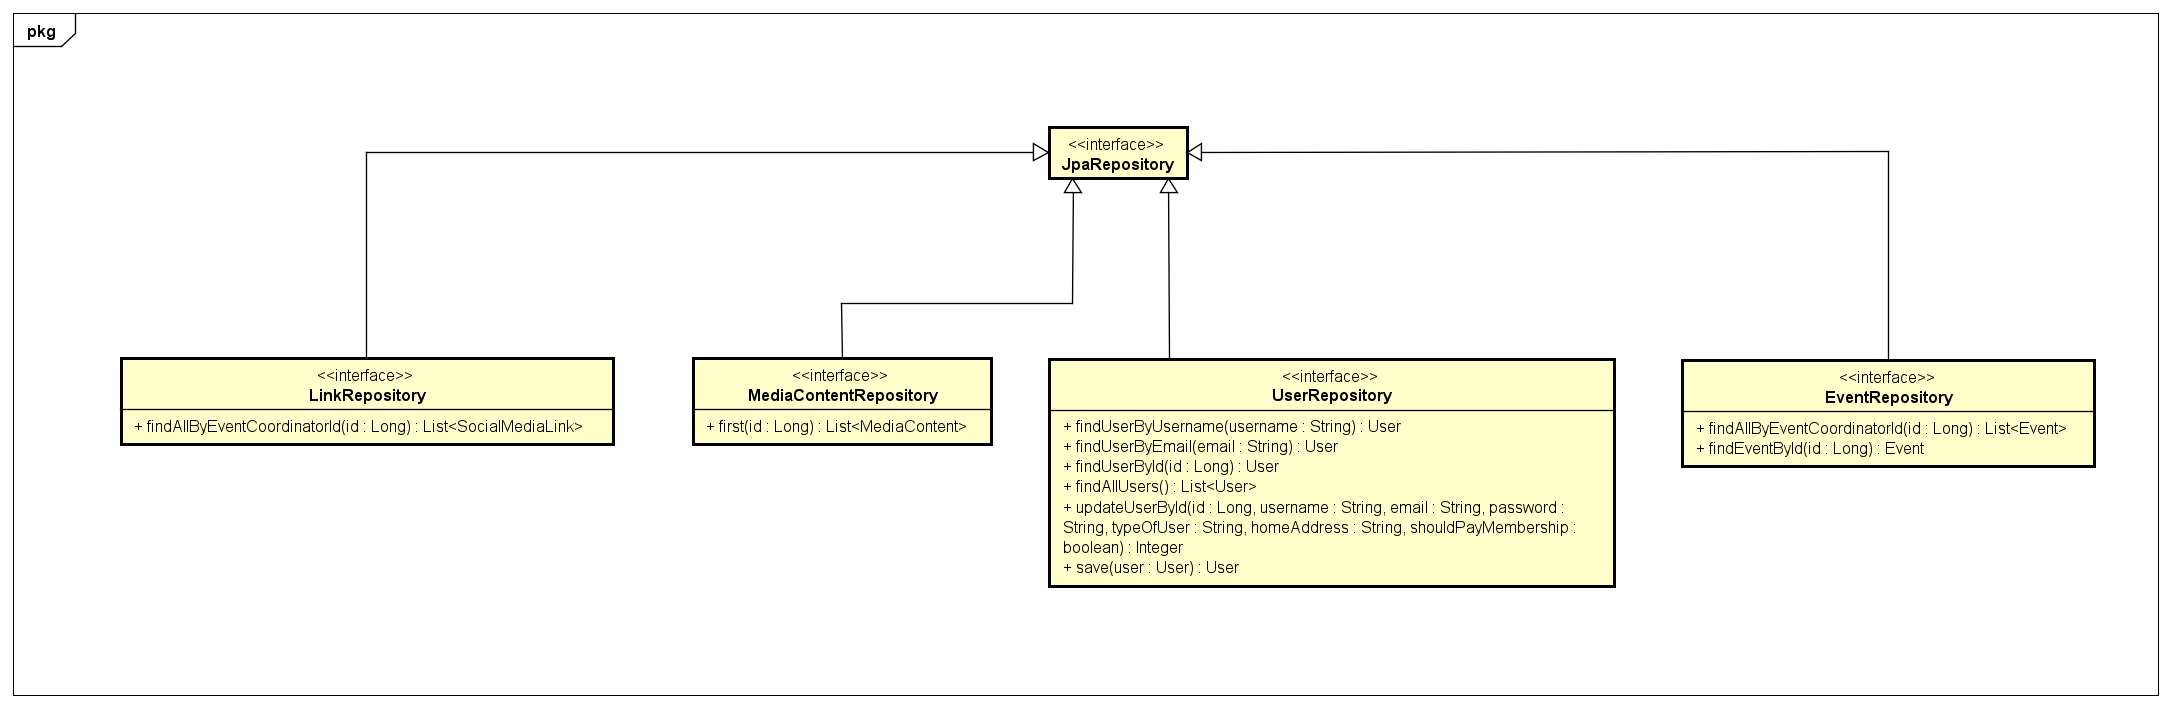
\includegraphics[width=\textwidth]{dijagrami/cd2.png} 
				\centering
				\vspace{-0.5cm}
				\caption{Dijagram razreda - Repository}
				\label{cd2}
			\end{figure}
			
			\begin{figure}[H]
				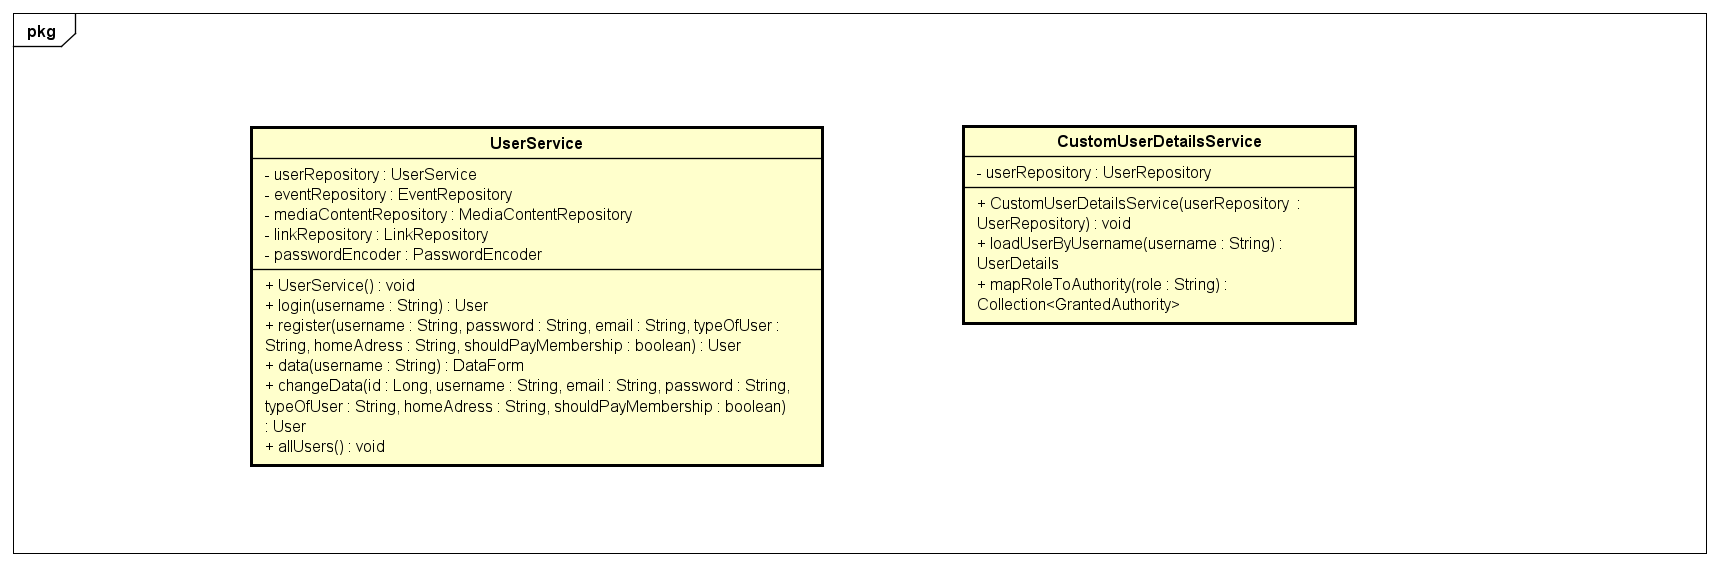
\includegraphics[width=\textwidth]{dijagrami/cd5.png} 
				\centering
				\vspace{-0.5cm}
				\caption{Dijagram razreda - Services}
				\label{cd5}
			\end{figure}
			
			\begin{figure}[H]
				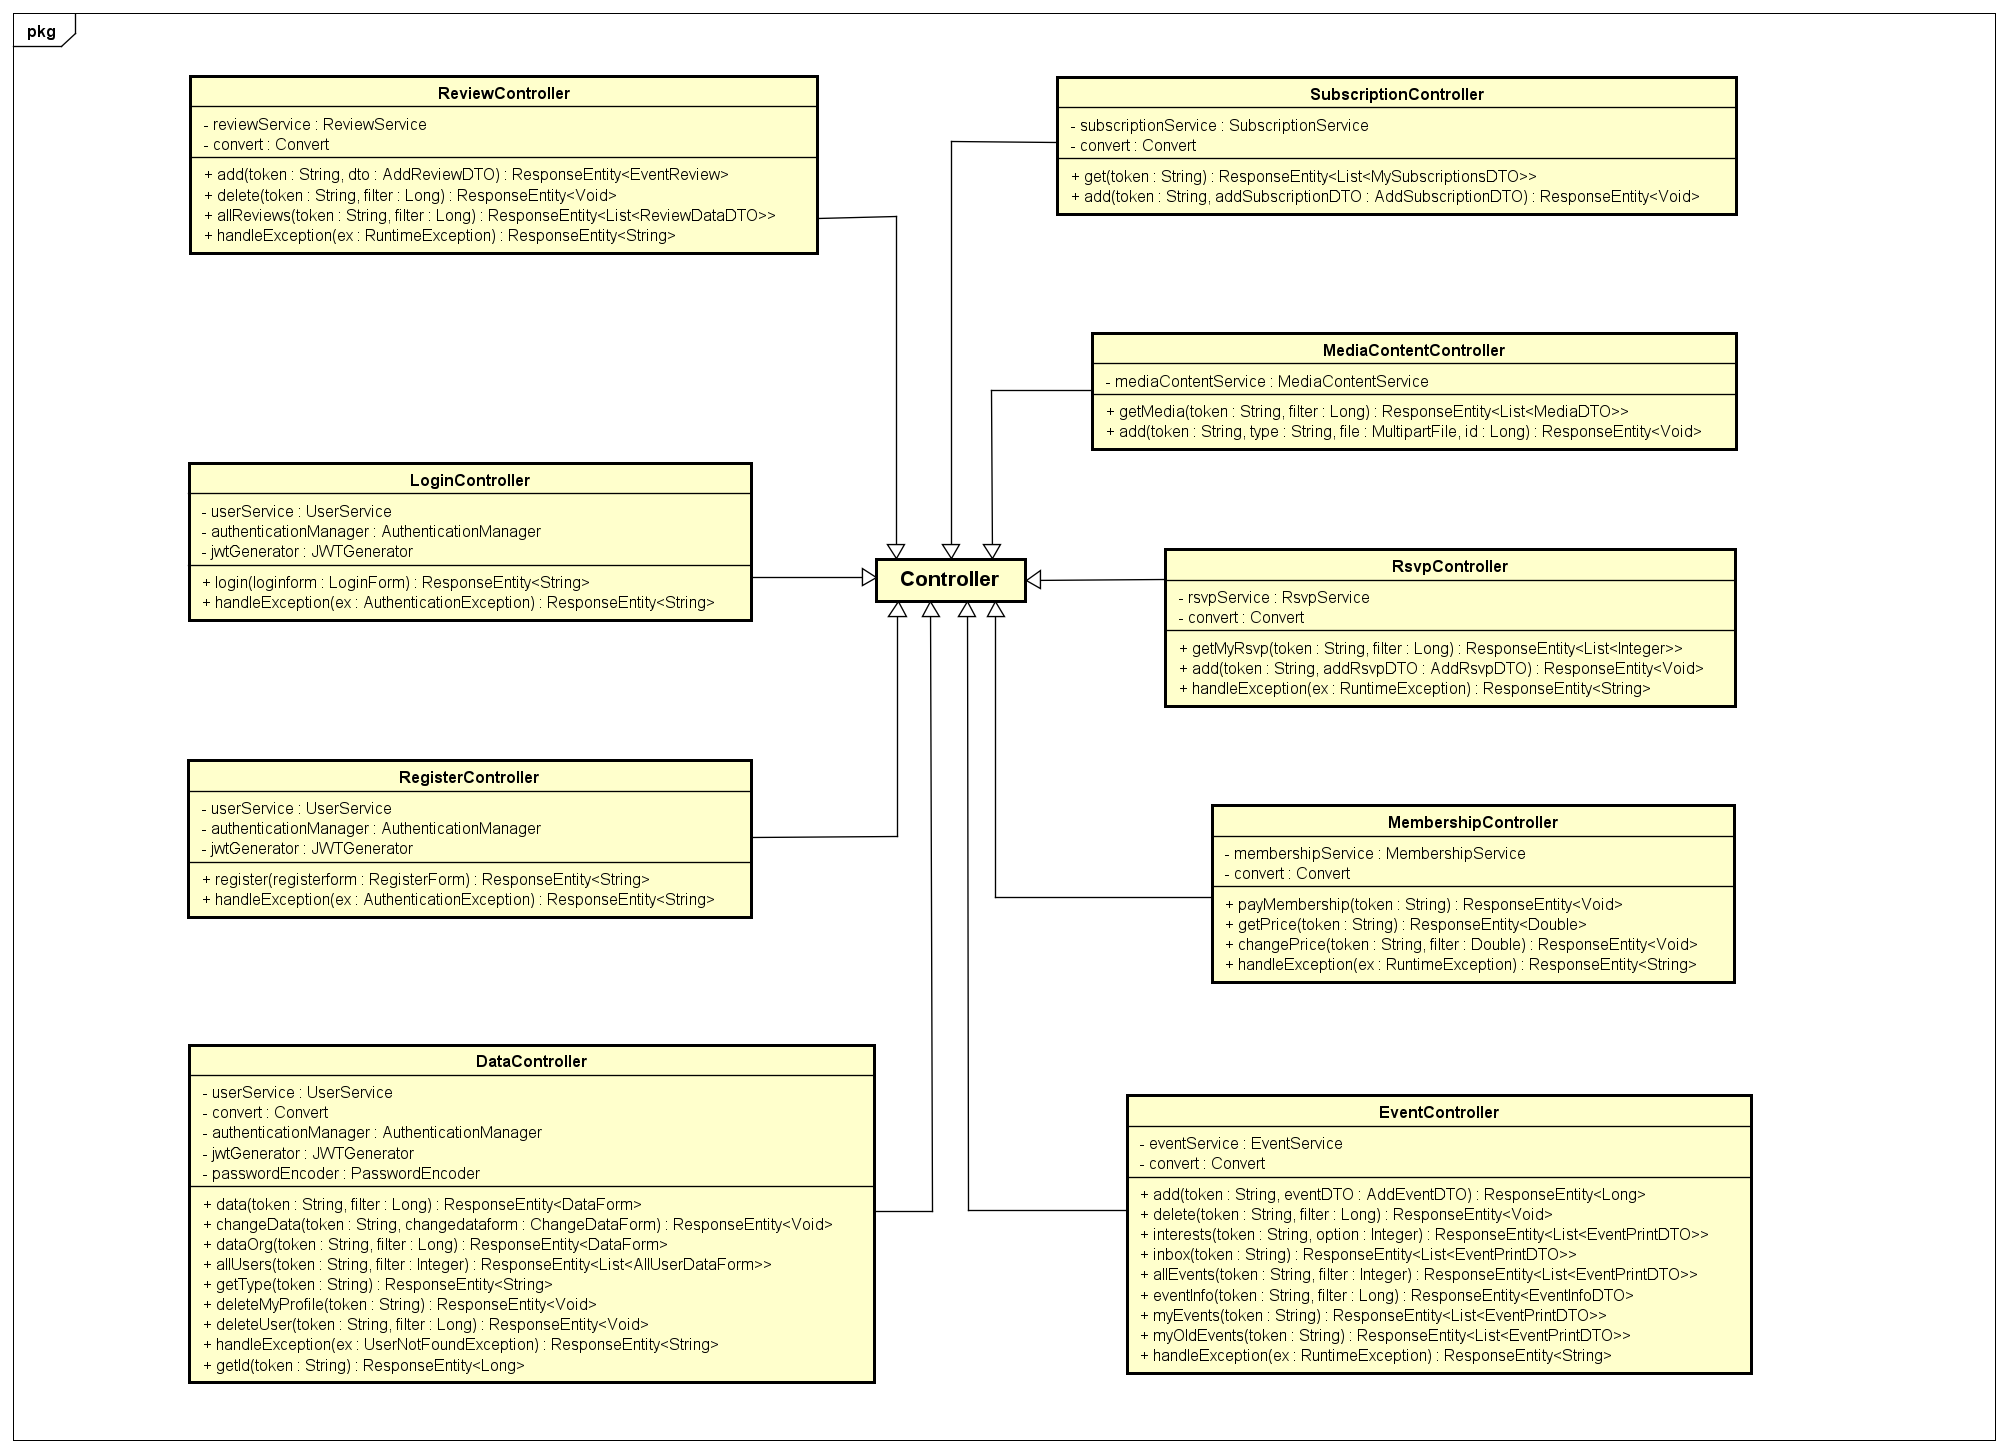
\includegraphics[width=\textwidth]{dijagrami/cd3.png} 
				\centering
				\vspace{-0.4cm}
				\caption{Dijagram razreda - Controllers}
				\label{cd3}
			\end{figure}
			
				
			
			
			\begin{figure}[H]
				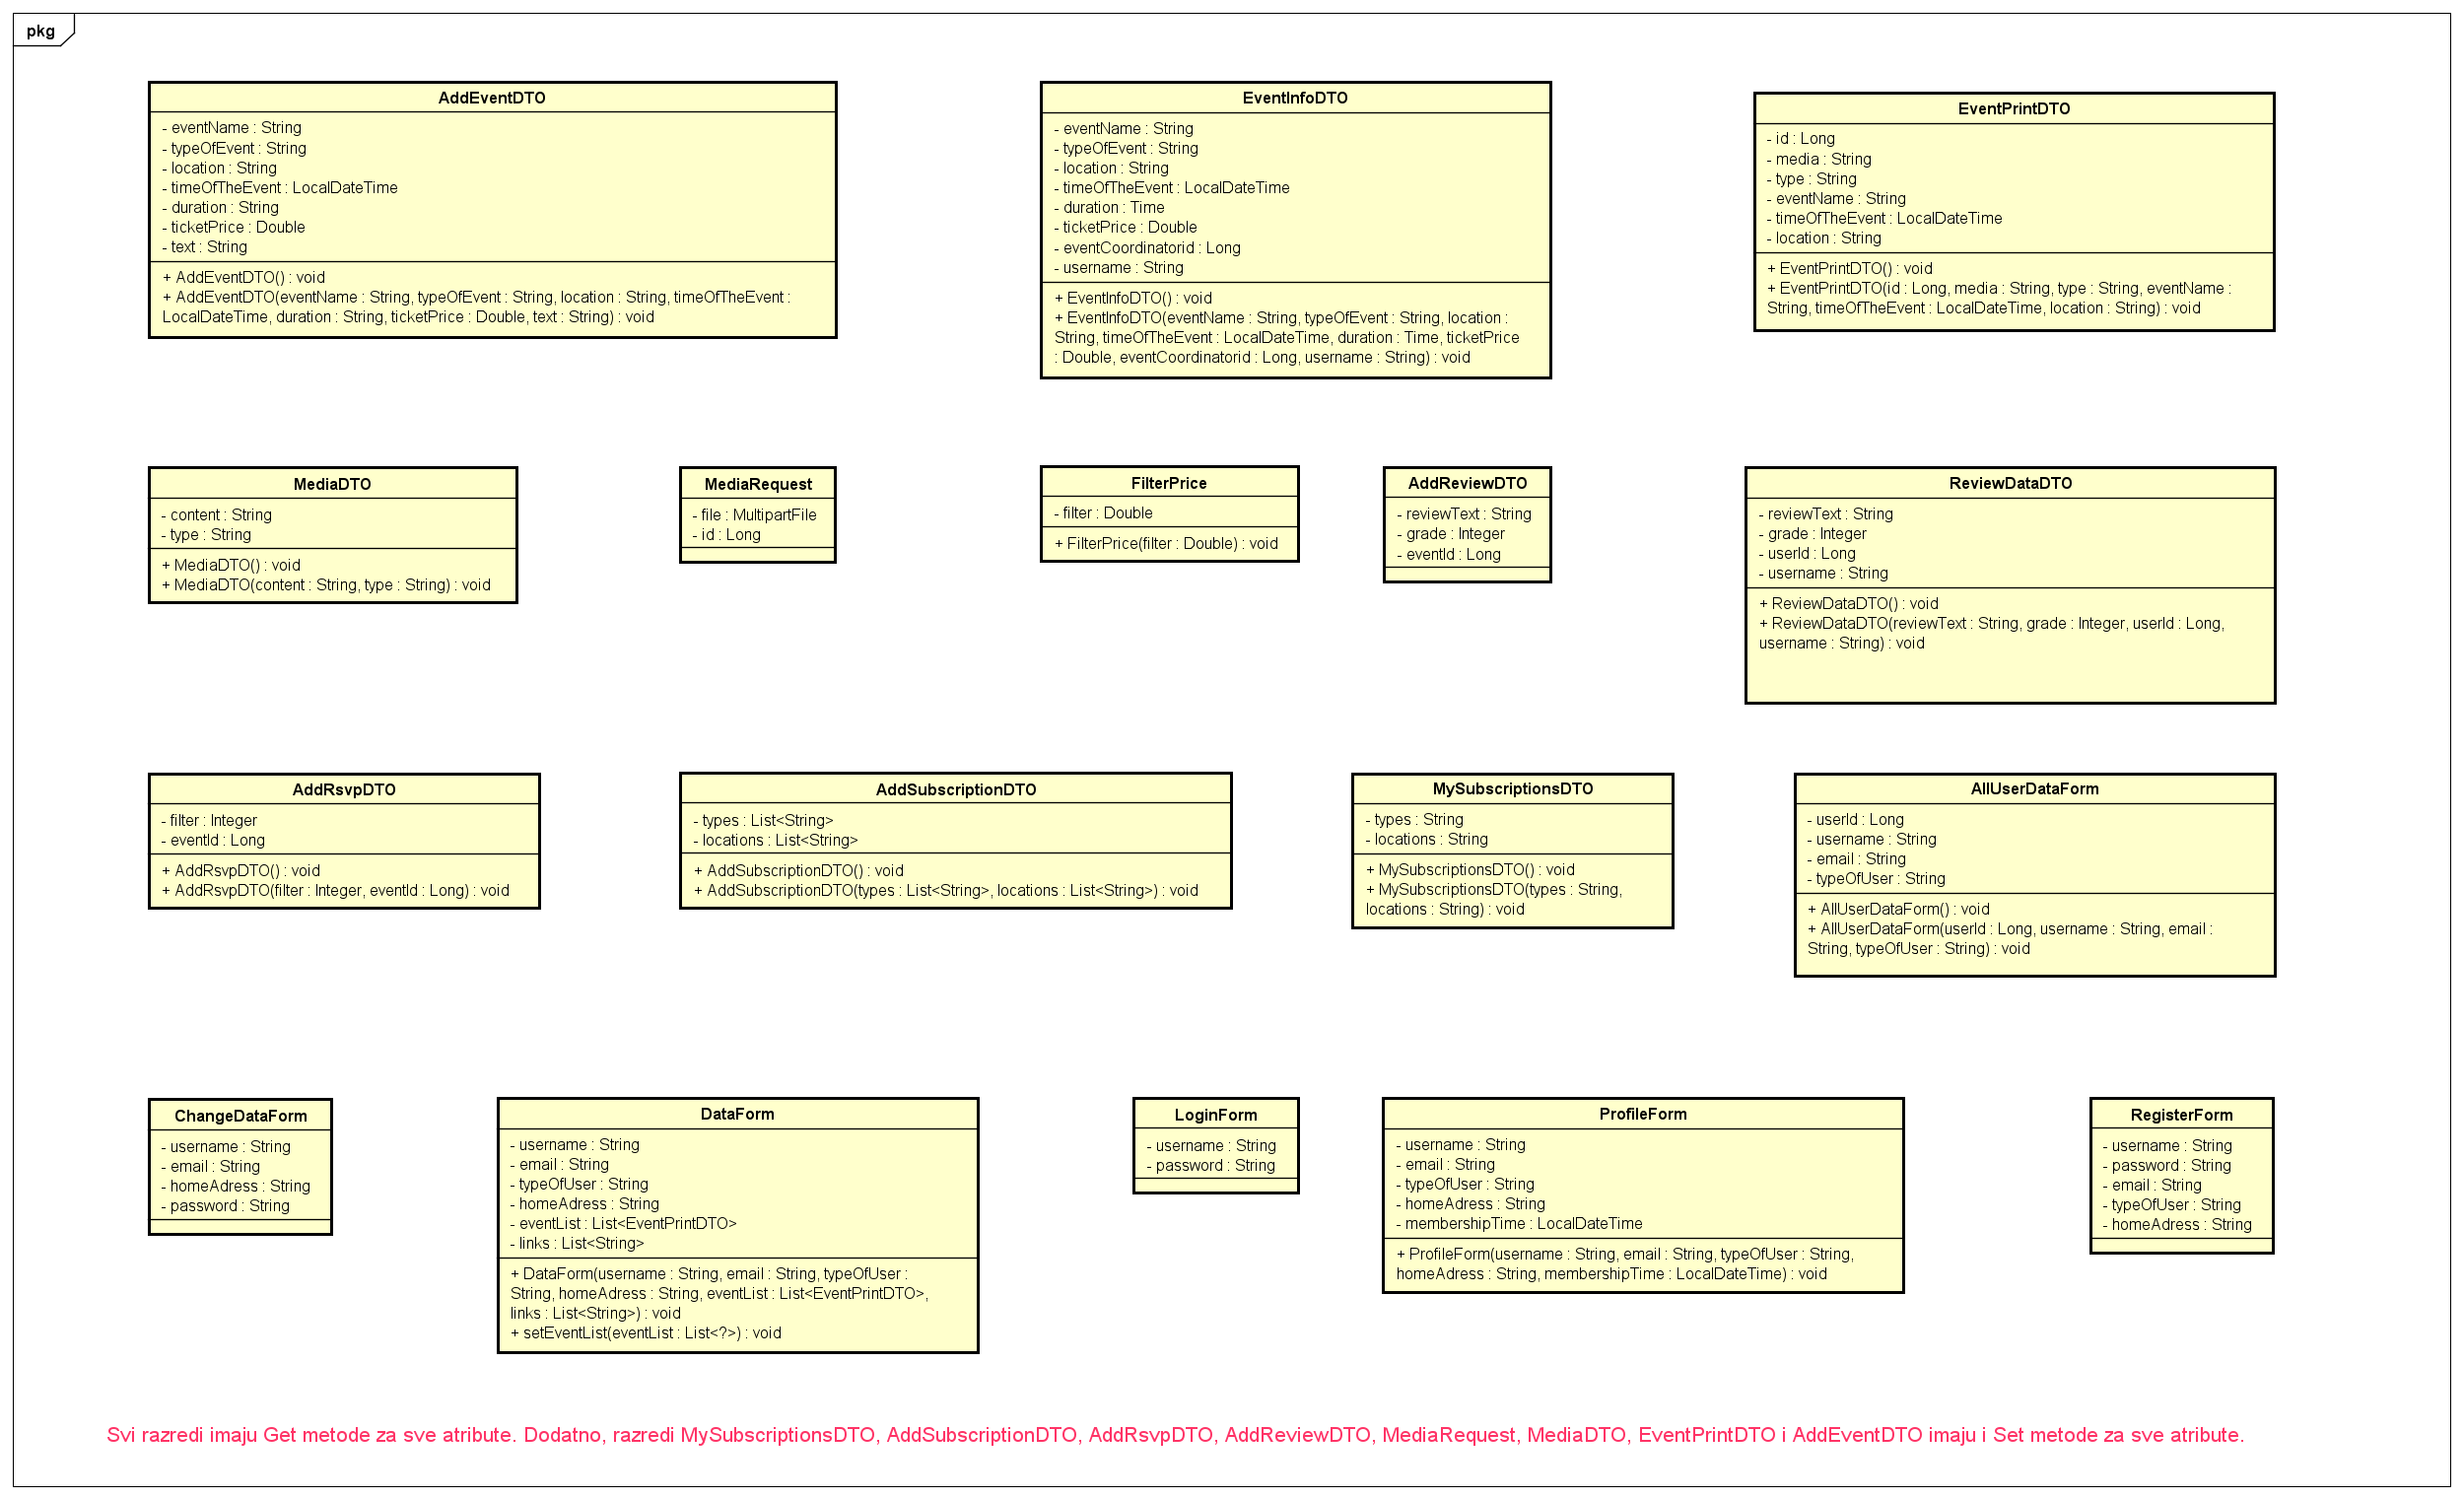
\includegraphics[width=\textwidth]{dijagrami/cd4.png} 
				\centering
				\vspace{-0.4cm}
				\caption{Dijagram razreda - Data transfer objects}
				\label{cd4}
			\end{figure}
			
		
			
			\newpage
			
			\begin{figure}[H]
				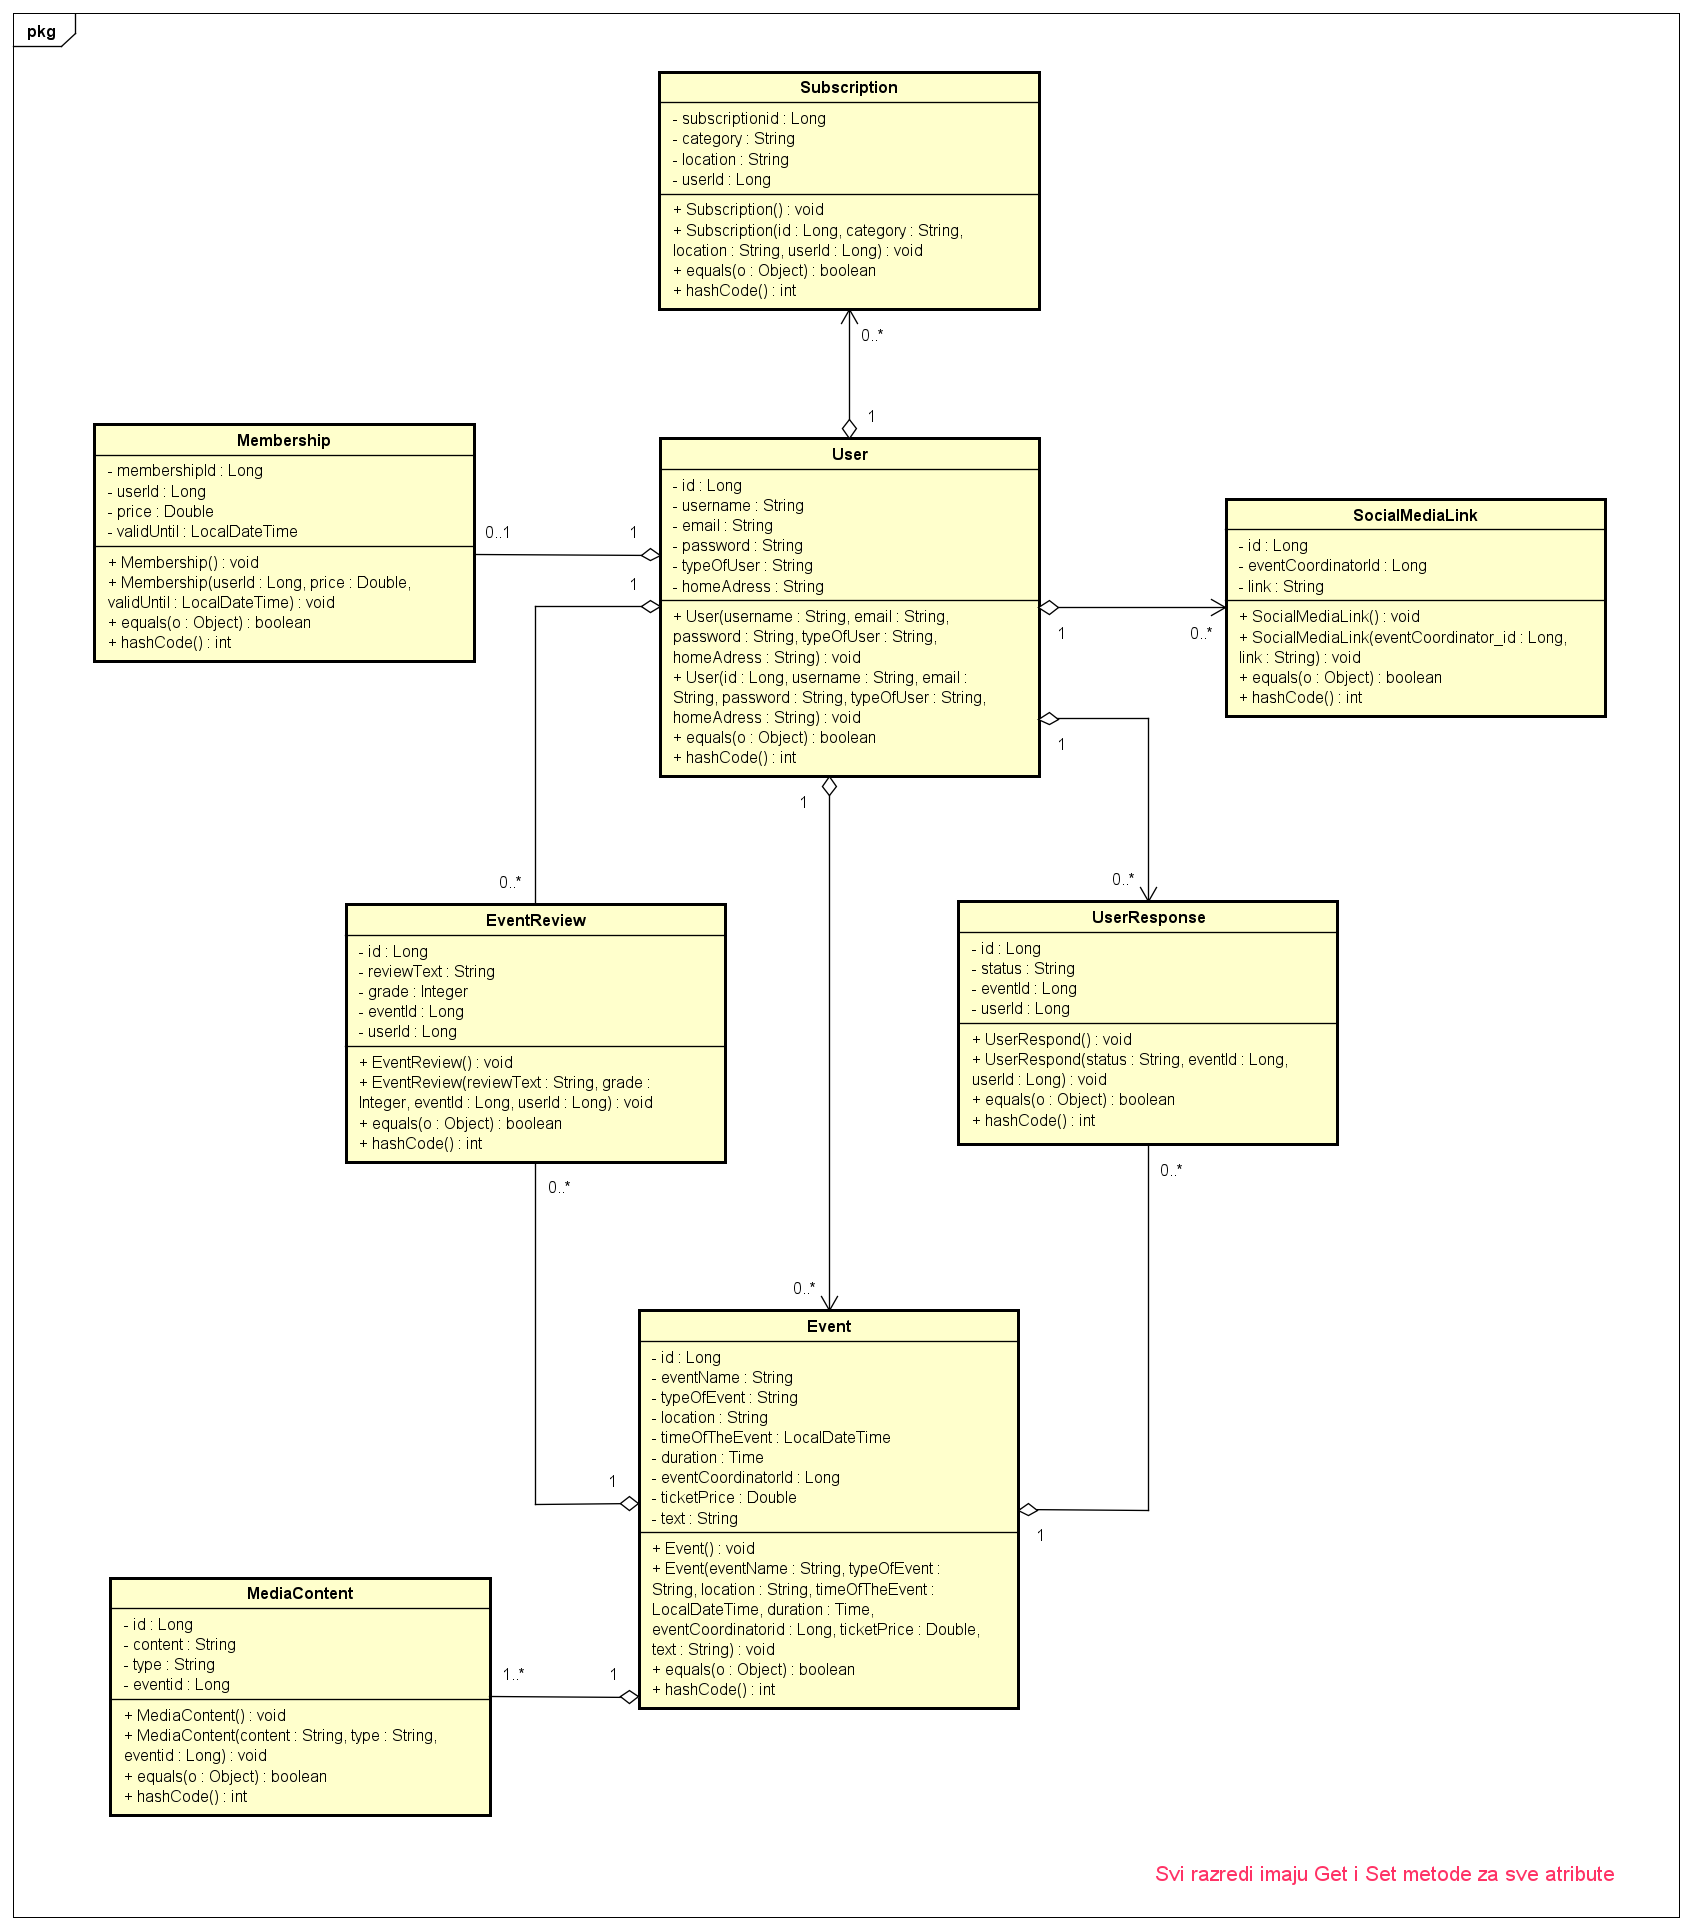
\includegraphics[width=\textwidth]{dijagrami/cd1.png} 
				\centering
				\caption{Dijagram razreda - Models}
				\label{cd1}
			\end{figure}

			\eject
		
		\section{Dijagram stanja}
			
			 Na slici \ref{sd} prikazan je dijagram stanja sustava za Posjetitelja i Organizatora. Neposredno nakon prijave u sustav, korisniku se prikazuje početna stranica sa osnovnim informacijama o web-aplikaciji. Ako je korisnik Posjetitelj, dostupne su mu opcije \textit{Početna stranica}, \textit{Događanja}, \textit{Inbox}, \textit{Zanima me}, \textit{Moj račun}, \textit{O nama} i \textit{Odjava}. Ako je korisnik ima ovlasti Organizatora, dodatno mu je dostupna opcija \textit{Moja događanja}. Biranjem opcije \textit{Moj račun} prikazuju se korisnički podaci i nude se opcije uređivanja osobnih podataka (opcija \textit{Uredi profil}), brisanje korisničkog računa i uređivanje postavki obavještavanja o novim događanjima (ta nova događanja pojavit će se u sekciji \textit{Inbox}). Organizatori na ovom mjestu, uz navedeno, imaju dodatnu opciju dodavanja novog događanja. Aktualna događanja prikazuju se odabirom opcije \textit{Događanja}, a moguće ih je i filtrirati prema vremenskom razdoblju.  Kad je iz popisa svih događanja odbrano i otvoreno jedno događanje, moguće ga je recenzirati, iskazati interes te prikazati profil organizatora događanja. Odabirom opcije \textit{Zanima me} prikazuju se događanja za koja je korisnik iskazao interes, a odabirom \textit{Moja događanja} organizatoru se prikazuju sva vlastita događanja. Odabirom opcije \textit{O nama} prikazuju se informacije o web-aplikaciji, a odabirom opcije \textit{Odjava} korisnik se odjavljuje iz sustava. 
				
			
			 \begin{figure}[H]
				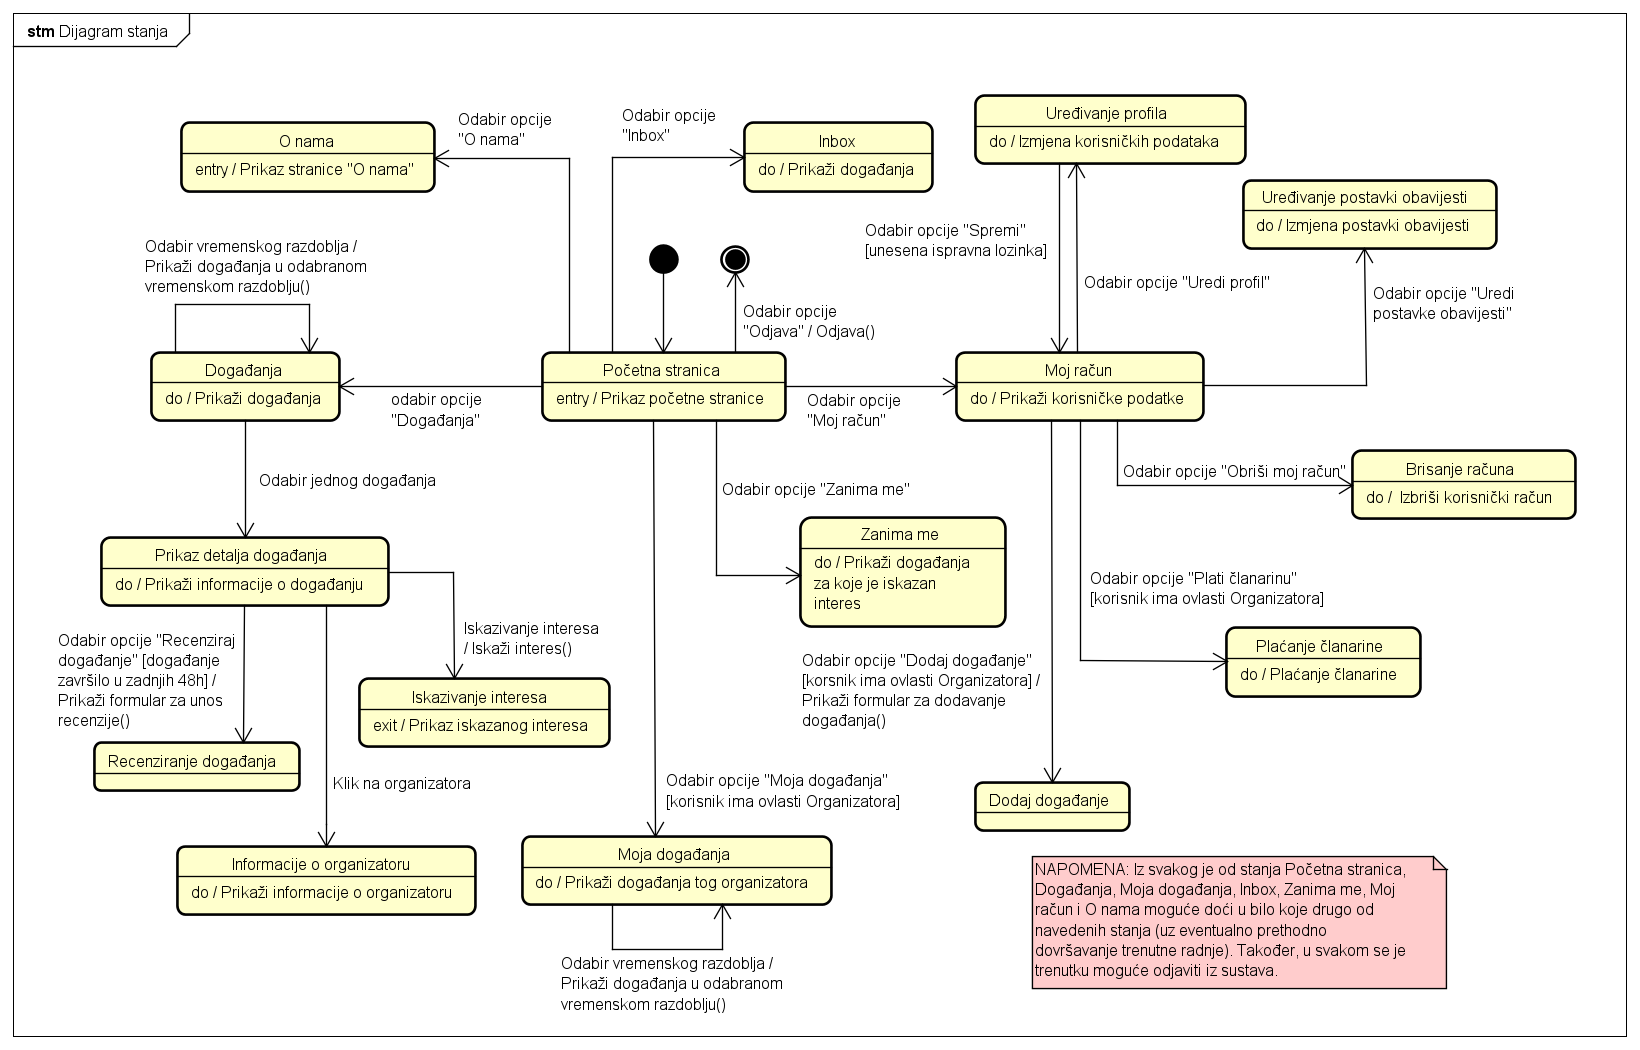
\includegraphics[width=\textwidth]{dijagrami/sd.png} 
				\centering
				\vspace{-0.75cm}
				\caption{Dijagram stanja}
				\label{sd}
			\end{figure}
			
			\eject 
		
		\section{Dijagram aktivnosti}
			
			
			 Slika \ref{ad} prikazuje dijagram aktivnosti za proces prijave korisnika u sustav, prikaz događanja u odabranom vremenskom razdoblju i opcionalni odabir neke od dodatnih opcija pri prikazu jednog događanja. Korisnik nakon uspješne prijave u sustav odabire opciju \textit{Događanja} nakon čega mu se prikazuju aktualna događanja. Prikazana događanja može i filtrirati po vremenskom razdoblju. Iz popisa događanja korisnik može odabrati jedno i dobiti prikaz detaljnih informacija o tom događanju. Na stranici sa podacima o odabranom događanju korisnik može odabrati i opcije prikaz profila organizatora, unos ocjene i recenzije za događanje te može iskazati interes za događanje. 
			 
			 \begin{figure}[H]
			 	\vspace{-0.8cm}
			 	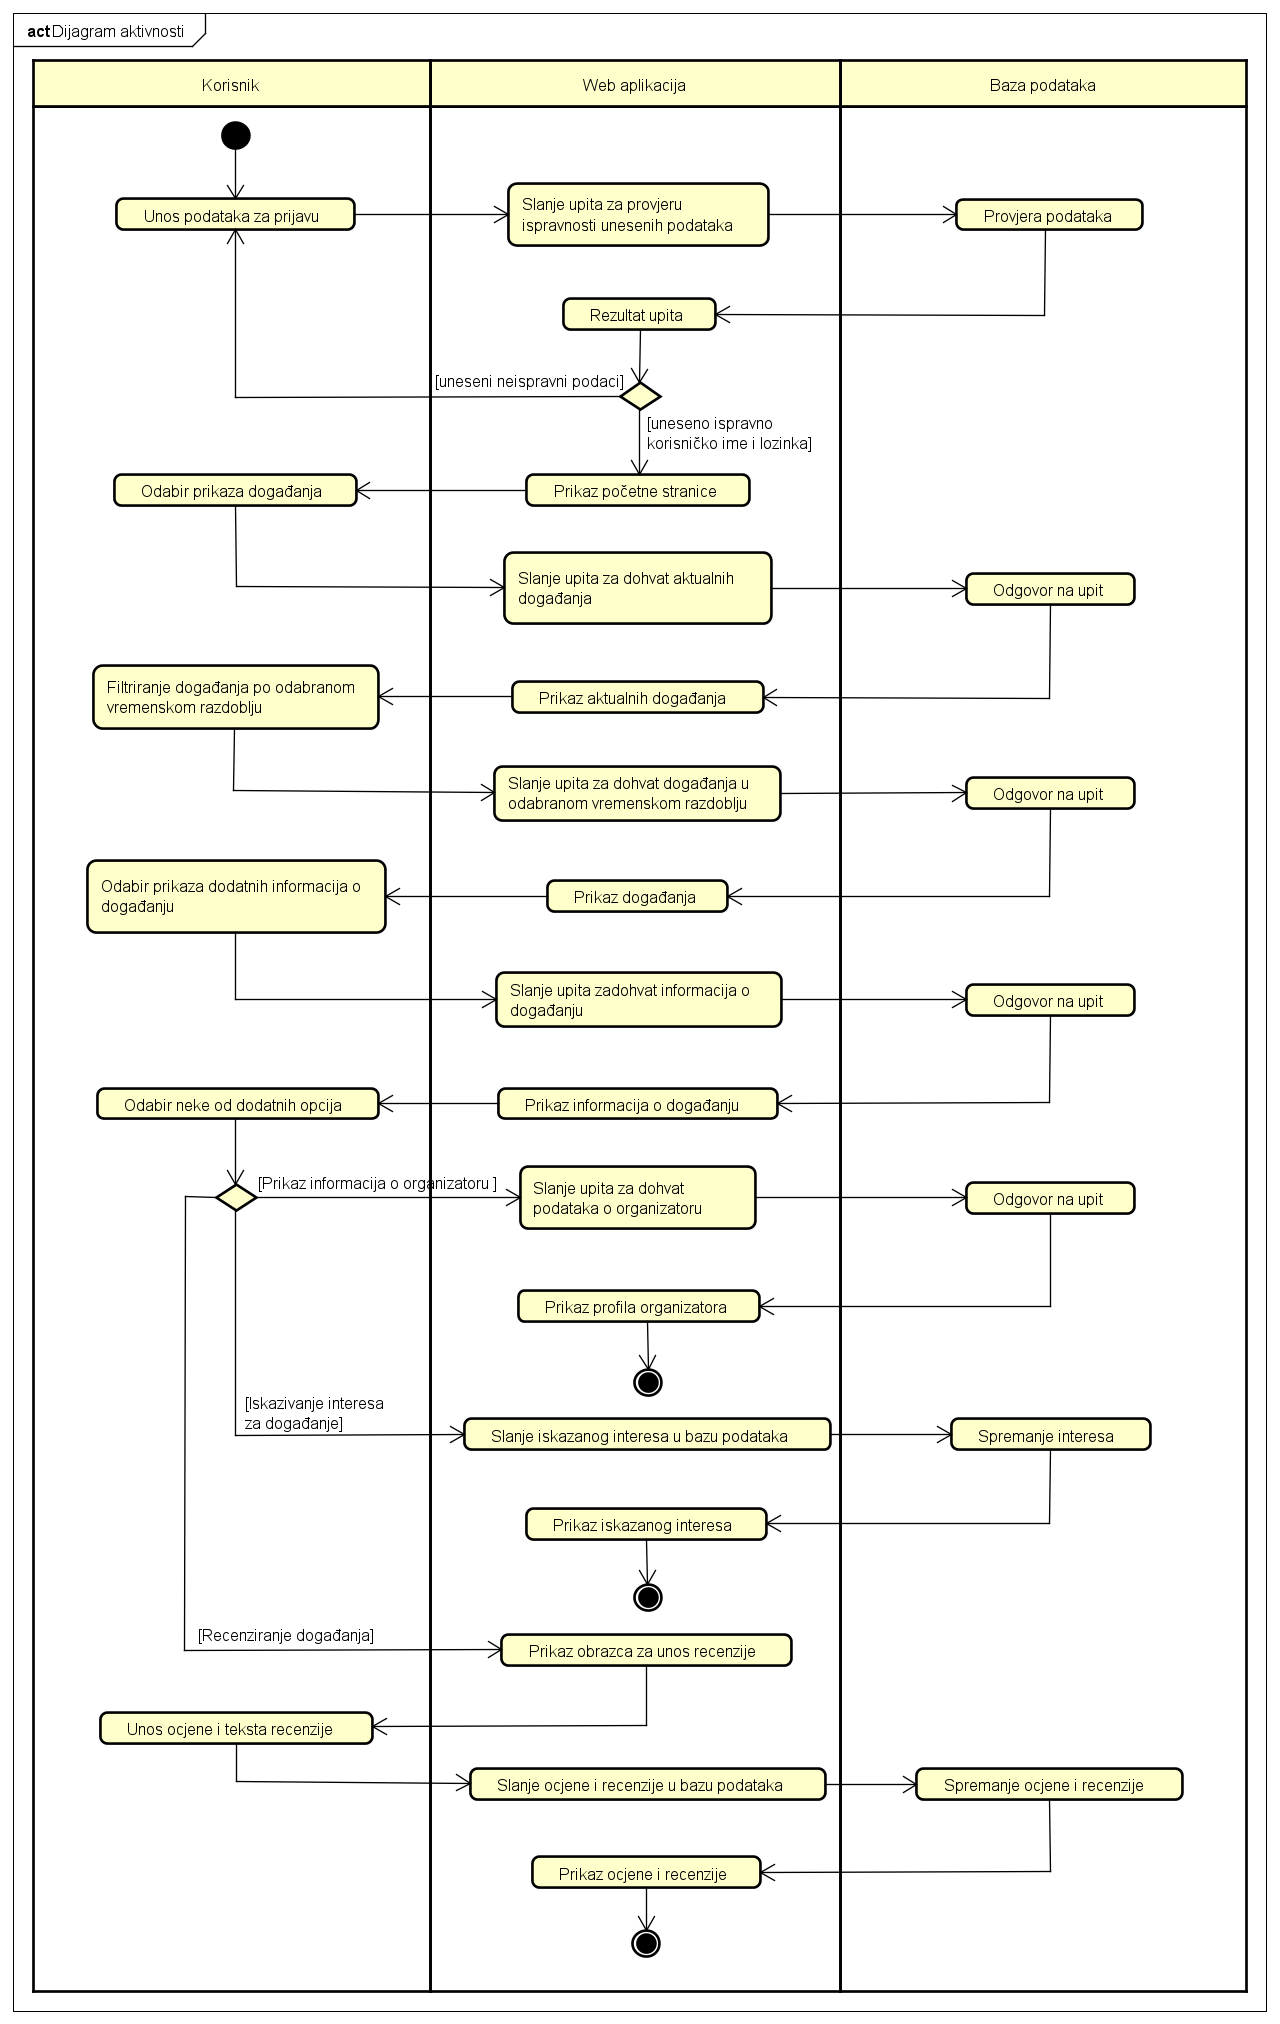
\includegraphics[width=\textwidth]{dijagrami/ad.png} 
			 	\centering
			 	\vspace{-1cm}
			 	\caption{Dijagram aktivnosti}
			 	\label{ad}
			 \end{figure}
			
			\eject
		\section{Dijagram komponenti}
		
			\textbf{\textit{dio 2. revizije}}\\
		
			 \textit{Potrebno je priložiti dijagram komponenti s pripadajućim opisom. Dijagram komponenti treba prikazivati strukturu cijele aplikacije.}
	\chapter{Implementacija i korisničko sučelje}
		
		
		\section{Korištene tehnologije i alati}
		
			\textbf{\textit{dio 2. revizije}}
			
			 \textit{Detaljno navesti sve tehnologije i alate koji su primijenjeni pri izradi dokumentacije i aplikacije. Ukratko ih opisati, te navesti njihovo značenje i mjesto primjene. Za svaki navedeni alat i tehnologiju je potrebno \textbf{navesti internet poveznicu} gdje se mogu preuzeti ili više saznati o njima}.
			
			
			\eject 
		
	
		\section{Ispitivanje programskog rješenja}
			
			\textbf{\textit{dio 2. revizije}}\\
			
			 \textit{U ovom poglavlju je potrebno opisati provedbu ispitivanja implementiranih funkcionalnosti na razini komponenti i na razini cijelog sustava s prikazom odabranih ispitnih slučajeva. Studenti trebaju ispitati temeljnu funkcionalnost i rubne uvjete.}
	
			
			\subsection{Ispitivanje komponenti}
			\textit{Potrebno je provesti ispitivanje jedinica (engl. unit testing) nad razredima koji implementiraju temeljne funkcionalnosti. Razraditi \textbf{minimalno 6 ispitnih slučajeva} u kojima će se ispitati redovni slučajevi, rubni uvjeti te izazivanje pogreške (engl. exception throwing). Poželjno je stvoriti i ispitni slučaj koji koristi funkcionalnosti koje nisu implementirane. Potrebno je priložiti izvorni kôd svih ispitnih slučajeva te prikaz rezultata izvođenja ispita u razvojnom okruženju (prolaz/pad ispita). }
			
			
			
			\subsection{Ispitivanje sustava}
			
			 \textit{Potrebno je provesti i opisati ispitivanje sustava koristeći radni okvir Selenium\footnote{\url{https://www.seleniumhq.org/}}. Razraditi \textbf{minimalno 4 ispitna slučaja} u kojima će se ispitati redovni slučajevi, rubni uvjeti te poziv funkcionalnosti koja nije implementirana/izaziva pogrešku kako bi se vidjelo na koji način sustav reagira kada nešto nije u potpunosti ostvareno. Ispitni slučaj se treba sastojati od ulaza (npr. korisničko ime i lozinka), očekivanog izlaza ili rezultata, koraka ispitivanja i dobivenog izlaza ili rezultata.\\ }
			 
			 \textit{Izradu ispitnih slučajeva pomoću radnog okvira Selenium moguće je provesti pomoću jednog od sljedeća dva alata:}
			 \begin{itemize}
			 	\item \textit{dodatak za preglednik \textbf{Selenium IDE} - snimanje korisnikovih akcija radi automatskog ponavljanja ispita	}
			 	\item \textit{\textbf{Selenium WebDriver} - podrška za pisanje ispita u jezicima Java, C\#, PHP koristeći posebno programsko sučelje.}
			 \end{itemize}
		 	\textit{Detalji o korištenju alata Selenium bit će prikazani na posebnom predavanju tijekom semestra.}
			
			\eject 
		
		
		\section{Dijagram razmještaja}
			
			\textbf{\textit{dio 2. revizije}}
			
			 \textit{Potrebno je umetnuti \textbf{specifikacijski} dijagram razmještaja i opisati ga. Moguće je umjesto specifikacijskog dijagrama razmještaja umetnuti dijagram razmještaja instanci, pod uvjetom da taj dijagram bolje opisuje neki važniji dio sustava.}
			
			\eject 
		
		\section{Upute za puštanje u pogon}
		
			\textbf{\textit{dio 2. revizije}}\\
		
			 \textit{U ovom poglavlju potrebno je dati upute za puštanje u pogon (engl. deployment) ostvarene aplikacije. Na primjer, za web aplikacije, opisati postupak kojim se od izvornog kôda dolazi do potpuno postavljene baze podataka i poslužitelja koji odgovara na upite korisnika. Za mobilnu aplikaciju, postupak kojim se aplikacija izgradi, te postavi na neku od trgovina. Za stolnu (engl. desktop) aplikaciju, postupak kojim se aplikacija instalira na računalo. Ukoliko mobilne i stolne aplikacije komuniciraju s poslužiteljem i/ili bazom podataka, opisati i postupak njihovog postavljanja. Pri izradi uputa preporučuje se \textbf{naglasiti korake instalacije uporabom natuknica} te koristiti što je više moguće \textbf{slike ekrana} (engl. screenshots) kako bi upute bile jasne i jednostavne za slijediti.}
			
			
			 \textit{Dovršenu aplikaciju potrebno je pokrenuti na javno dostupnom poslužitelju. Studentima se preporuča korištenje neke od sljedećih besplatnih usluga: \href{https://aws.amazon.com/}{Amazon AWS}, \href{https://azure.microsoft.com/en-us/}{Microsoft Azure} ili \href{https://www.heroku.com/}{Heroku}. Mobilne aplikacije trebaju biti objavljene na F-Droid, Google Play ili Amazon App trgovini.}
			
			
			\eject 
	\chapter{Zaključak i budući rad}
		
		\textbf{\textit{dio 2. revizije}}\\
		
		 \textit{U ovom poglavlju potrebno je napisati osvrt na vrijeme izrade projektnog zadatka, koji su tehnički izazovi prepoznati, jesu li riješeni ili kako bi mogli biti riješeni, koja su znanja stečena pri izradi projekta, koja bi znanja bila posebno potrebna za brže i kvalitetnije ostvarenje projekta i koje bi bile perspektive za nastavak rada u projektnoj grupi.}
		
		 \textit{Potrebno je točno popisati funkcionalnosti koje nisu implementirane u ostvarenoj aplikaciji.}
		
		\eject 
	\chapter*{Popis literature}
		\addcontentsline{toc}{chapter}{Popis literature}
		
		
		\begin{enumerate}
			
			
			\item  Programsko inženjerstvo, FER ZEMRIS, \url{https://www.fer.unizg.hr/predmet/proinz}
			
			\item  I. Sommerville, "Software engineering", 8th ed, Addison Wesley, 2007.
			
			\item  T.C.Lethbridge, R.Langaniere, "Object-Oriented Software Engineering", 2nd ed. McGraw-Hill, 2005.
			
			\item  I. Marsic, Software engineering book``, Department of Electrical and Computer Engineering, Rutgers University, \url{http://www.ece.rutgers.edu/~marsic/books/SE}
			
			\item  The Unified Modeling Language, \url{https://www.uml-diagrams.org/}
			
			\item  Astah Community, \url{http://astah.net/editions/uml-new}
		\end{enumerate}
		
		 
	
	
	\begingroup
	\renewcommand*\listfigurename{Indeks slika i dijagrama}
	%\renewcommand*\listtablename{Indeks tablica}
	%\let\clearpage\relax
	\listoffigures
	%\vspace{10mm}
	%\listoftables
	\endgroup
	\addcontentsline{toc}{chapter}{Indeks slika i dijagrama}


	
	\eject 
		
	\chapter*{Dodatak: Prikaz aktivnosti grupe}
		\addcontentsline{toc}{chapter}{Dodatak: Prikaz aktivnosti grupe}
		
		\section*{Dnevnik sastajanja}
		
		\begin{packed_enum}
			\item  sastanak
			
			\item[] \begin{packed_item}
				\item Datum: 19. listopada 2023.
				\item Prisustvovali: L. Topolko, J. Kolarec, I.Svalina, I. Kvesić, N. Lazarić, F. Mišković, B. Marković
				\item Teme sastanka:
				\begin{packed_item}
					\item dogovor o korištenim tehnologijama
					\item dogovor o načinima komunikacije
					\item podjela u timove za frontend, backend i dokumentaciju
					\item definiranje osnovnih funkcionalnosti
				\end{packed_item}
			\end{packed_item}
			
			\item  sastanak
			\item[] \begin{packed_item}
				\item Datum: 23. listopada 2023.
				\item Prisustvovali: L. Topolko, J. Kolarec, I.Svalina, I. Kvesić, N. Lazarić, F. Mišković, B. Marković
				\item Teme sastanka:
				\begin{packed_item}
					\item sastavljanje use-caseova
					\item razgovor o povezivanju frontenda i backenda
					\item dogovor o bazi i sadržaju baze
				\end{packed_item}
			\end{packed_item}
			
			\item  sastanak
			\item[] \begin{packed_item}
				\item Datum: 24. listopada 2023.
				\item Prisustvovali: L. Topolko, N. Lazarić, I. Svalina
				\item Teme sastanka:
				\begin{packed_item}
					\item  osmišljavanje baze podataka (odabir h2 baze za lokalno testiranje, odabir entiteta i njihovih atributa)
				\end{packed_item}
			\end{packed_item}
			
			\item  sastanak
			\item[] \begin{packed_item}
				\item Datum: 26. listopada 2023.
				\item Prisustvovali: F. Mišković, I. Kvesić, B. Marković
				\item Teme sastanka:
				\begin{packed_item}
					\item  dogovor o podjeli posla
					\item  određen okvirni izgled stranice
				\end{packed_item}
			\end{packed_item}
		
		
			\item  sastanak
			\item[] \begin{packed_item}
				\item Datum: 9. studenoga 2023.
				\item Prisustvovali: L. Topolko, J. Kolarec, I. Kvesić, N. Lazarić, F. Mišković, B. Marković
				\item Teme sastanka:
				\begin{packed_item}
					\item  od nastavnice dobivena povratna informacija o dosadašnjem radu 
					\item  utvrđivanje zadataka koje je potrebno dovršiti do prve predaje 
					\item dogovor o budućem izgledu pojedinih stranica web aplikacije
				\end{packed_item}
			\end{packed_item}
			
			
			\item  sastanak
			\item[] \begin{packed_item}
				\item Datum: 7. prosinca 2023.
				\item Prisustvovali: L. Topolko, J. Kolarec, I. Kvesić, N. Lazarić, B. Marković
				\item Teme sastanka:
				\begin{packed_item}
					\item dodjela bodova ostvarenih prilikom prve predaje projekta
				\end{packed_item}
			\end{packed_item}
			
			
			
			\item  sastanak
			\item[] \begin{packed_item}
				\item Datum: 11. siječnja 2024.
				\item Prisustvovali: L. Topolko, J. Kolarec, I. Svalina, I. Kvesić, N. Lazarić, F. Mišković, B. Marković
				\item Teme sastanka:
				\begin{packed_item}
					\item kontrolna točka prije konačne predaje projekta
					\item uputa i dogovor o daljnjem radu do predaje 
				\end{packed_item}
			\end{packed_item}
			
			
			\item  sastanak
			\item[] \begin{packed_item}
				\item Datum: 16. siječnja 2024.
				\item Prisustvovali: L. Topolko, J. Kolarec, I. Svalina, I. Kvesić, N. Lazarić, F. Mišković, B. Marković
				\item Teme sastanka:
				\begin{packed_item}
					\item podjela zadataka vezanih za prezentaciju projekta
					\item prezentacija i objašnjavanje vlastitih zadataka pojedinog člana tima ostalim članovima 
				\end{packed_item}
			\end{packed_item}
			
		
		
		\end{packed_enum}
		
		
		
		\eject
		\section*{Tablica aktivnosti}
		
			\vspace{-0.1cm}
			
			U tablici su navedeni doprinosi članova grupe u satima po pojedinoj aktivnosti. 
		
			\begin{longtblr}[
					label=none,
				]{
					vlines,hlines,
					width = \textwidth,
					colspec={X[7, l]X[1, c]X[1, c]X[1, c]X[1, c]X[1, c]X[1, c]X[1, c]}, 
					vline{1} = {1}{text=\clap{}},
					hline{1} = {1}{text=\clap{}},
					rowhead = 1,
				} 
			
				\SetCell[c=1]{c}{} & \SetCell[c=1]{c}{\rotatebox{90}{\textbf{Lucija Topolko}}} & \SetCell[c=1]{c}{\rotatebox{90}{\textbf{Natali Lazarić}}} &	\SetCell[c=1]{c}{\rotatebox{90}{\textbf{Julijana Kolarec }}} & \SetCell[c=1]{c}{\rotatebox{90}{\textbf{Iva Kvesić }}} &	\SetCell[c=1]{c}{\rotatebox{90}{\textbf{Bruno Marković}}} & \SetCell[c=1]{c}{\rotatebox{90}{\textbf{Filip Mišković}}} &	\SetCell[c=1]{c}{\rotatebox{90}{\textbf{Iva Svalina}}} \\  
				Upravljanje projektom 		& 7 &  &  &  &  &  & \\
				Sastanci  					& 6 & 6 & 6 & 6 & 6 & 6 & 6 \\ 
				Opis projektnog zadatka 	& 3 &  &  &  &  &  & \\ 
				
				Funkcionalni zahtjevi       & 1 &  & 2 &  &  &  &  \\ 
				Opis pojedinih obrazaca 	&  &  & 8 &  &  &  &  \\ 
				Dijagram obrazaca 			&  &  & 3 &  &  &  &  \\ 
				Sekvencijski dijagrami 		&  &  & 3 &  &  &  &  \\ 
				Opis ostalih zahtjeva 		&  &  & 1 &  &  &  &  \\ 

				Arhitektura i dizajn sustava	 &  &  & 2 &  &  &  &  \\ 
				Baza podataka				&  &  & 3 &  &  &  &   2\\ 
				Dijagram razreda 			& 2 &  & 7 &  &  &  &   \\ 
				Dodatak	 		 			&  &  & 1 &  &  &  &   \\
				Pravopis, čitljivost, opći dojam &  &  & 2 &  &  &  &   \\ 
				Backend & 10 & 12 &  &  &  &  &   \\ 
				Security  & 2 &  &  &  &  &  & 8 \\ 
				Deployment  & 20 & 22 &  &  &  &  & 15\\ 
				Istraživanje  & 2 & 1 &  1 & 8 & 8 & 8 & 10 \\ 
				Izrada baze podataka  & 2 &  &  &  &  &  & 3 \\ 
				Spajanje s bazom podataka
				 & 3 &  &  & 7 & 3 & 8  & 1  \\ 
				Izrada početne stranice  &  &  &  & 5 & 1 & 1 &   \\ 
				Izrada navigacijske trake  &  &  &  & 10 &  & 2 &   \\ 
				Izrada stranice za prijavu  &  &  &  &  & 13 & 2 &   \\ 
				\textbf{Ukupno do 1. revizije:} & \textbf{58} & \textbf{41}  & \textbf{39} & \textbf{36} & \textbf{31} & \textbf{27} & \textbf{45} \\ \hline 
				Upravljanje projektom		& 10 &  &  &  &  &  &  \\
				Sastanci  					& 4 & 4 & 4 & 4 & 4 & 4 & 4 \\  
				Dijagram razreda 			&  &  & 6 &  &  &  &  \\
				Dijagram stanja				&  &  & 3 &  &  &  &  \\ 
				Dijagram aktivnosti 		&  &  & 2 &  &  &  &  \\ 
				Dijagram komponenti			&  &  & 2 &  &  &  &  \\ 
				Korištene tehnologije i alati 		& 1 &  &  &  &  &  &  \\ 
				Ispitivanje programskog rj.	&  &  & 1 &  &  &  & 7  \\ 
				Dijagram razmještaja			&  &  & 1 &  &  &  &  \\ 
				Upute za puštanje u pogon 		&  & 3 &  &  &  &  &  \\  
				Dodatak 			&  &  & 2 &  &  &  &  \\ 
				Zaključak i budući rad 		&  &  & 1 &  &  &  &  \\  
				Revizija dokumentacije 		& 3 &  & 2 &  &  &  &  \\  
				Pravopis, čitljivost, opći dojam &  &  & 1 &  &  &  &  \\ 
				Istraživanje   					&  &  &  &  &  &  &  5\\ 
				Nadopuna baze podataka 			& 2 &  &  &  &  &  &  1\\  
				Backend  						& 12 & 12 &  &  &  &  &  \\ 
				Spremanje slika na cloud  		& 2 &  &  &  &  &  & 2 \\ 
				Frontend				  		& 7 &  & 2 & 26 & 29 & 30 &  \\
				Deployment  					& 5 &  &  &  &  &  &  \\
				Security  					&  &  &  &  &  &  &  16\\
				
				\textbf{Ukupno od 1. do 2. revizije:} & \textbf{46} & \textbf{19}  & \textbf{27} & \textbf{30} & \textbf{33} & \textbf{34} & \textbf{35} \\ \hline
				\textbf{SVEUKUPNO:}		& \textbf{104} & \textbf{60} & \textbf{66} & \textbf{66} & \textbf{64} & \textbf{61} & \textbf{80} \\
				
			\end{longtblr}
					
					
		\eject
		\section*{Dijagrami pregleda promjena}
		
		\begin{figure}[H]
			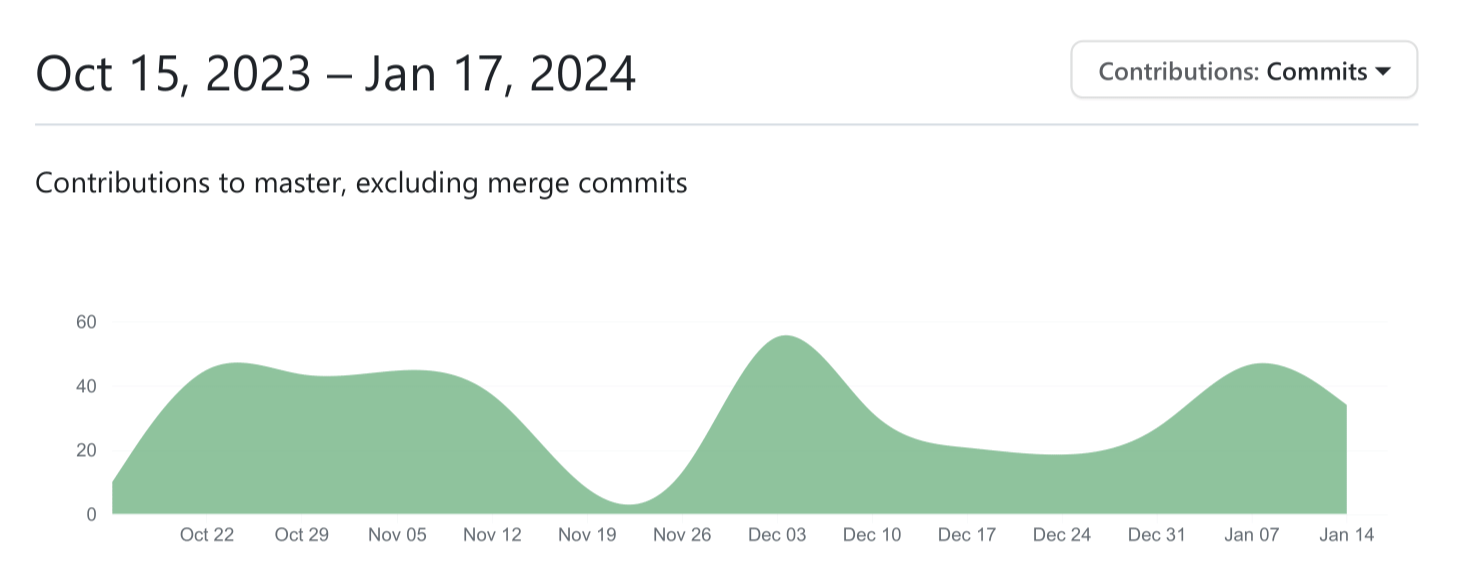
\includegraphics[width=\textwidth]{slike/promjene.png}
		\end{figure}
		
		\begin{figure}[H]
			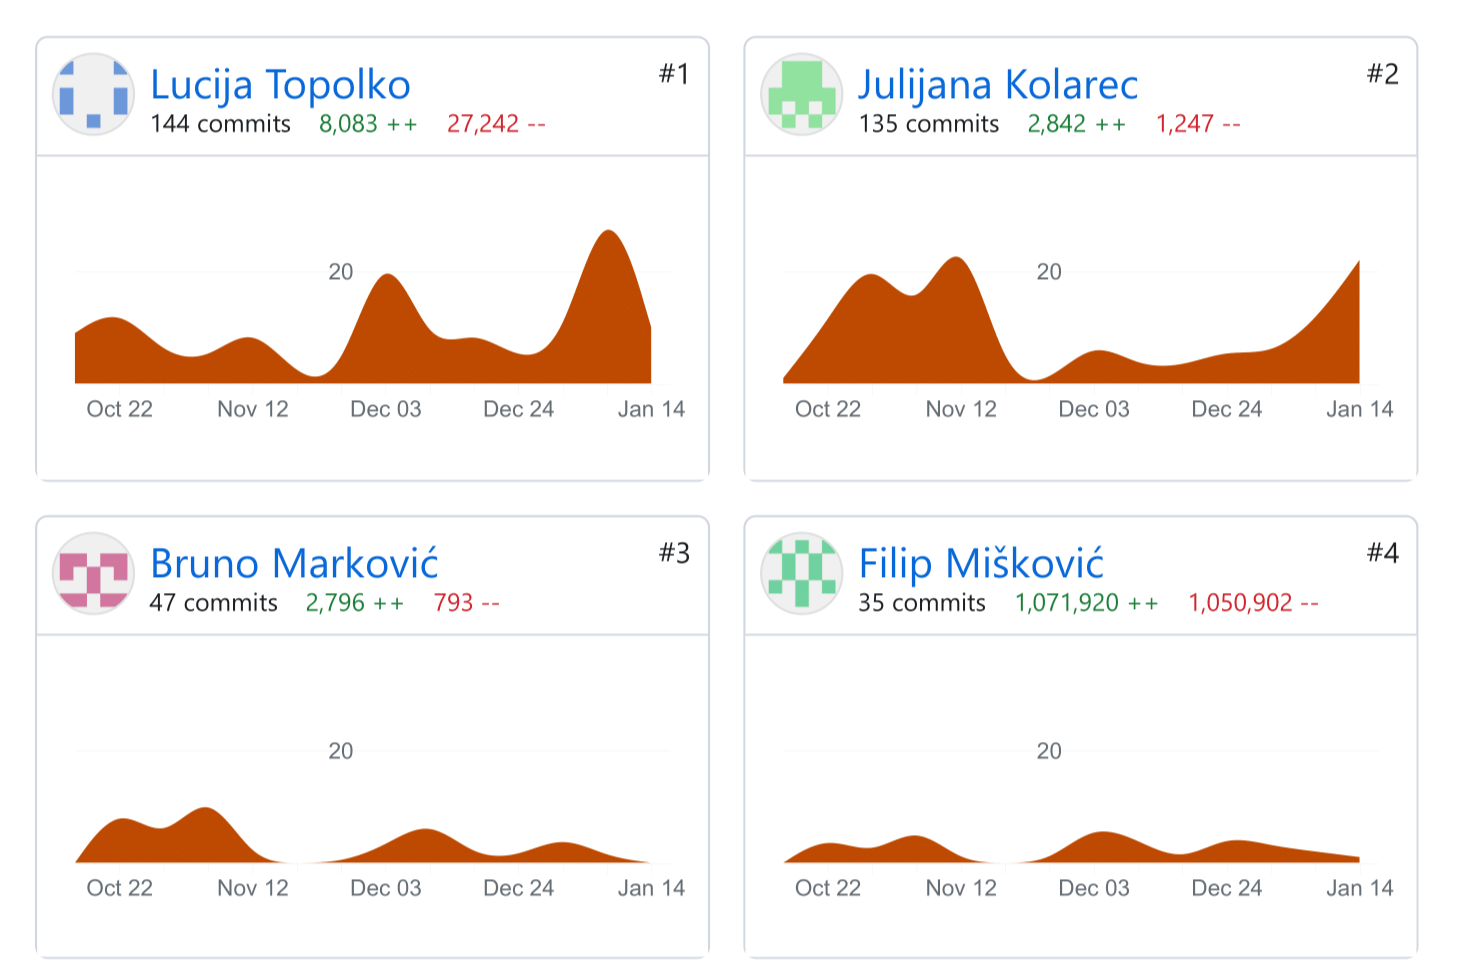
\includegraphics[width=\textwidth]{slike/promjene1.png}
		\end{figure}
		
			\begin{figure}[H]
			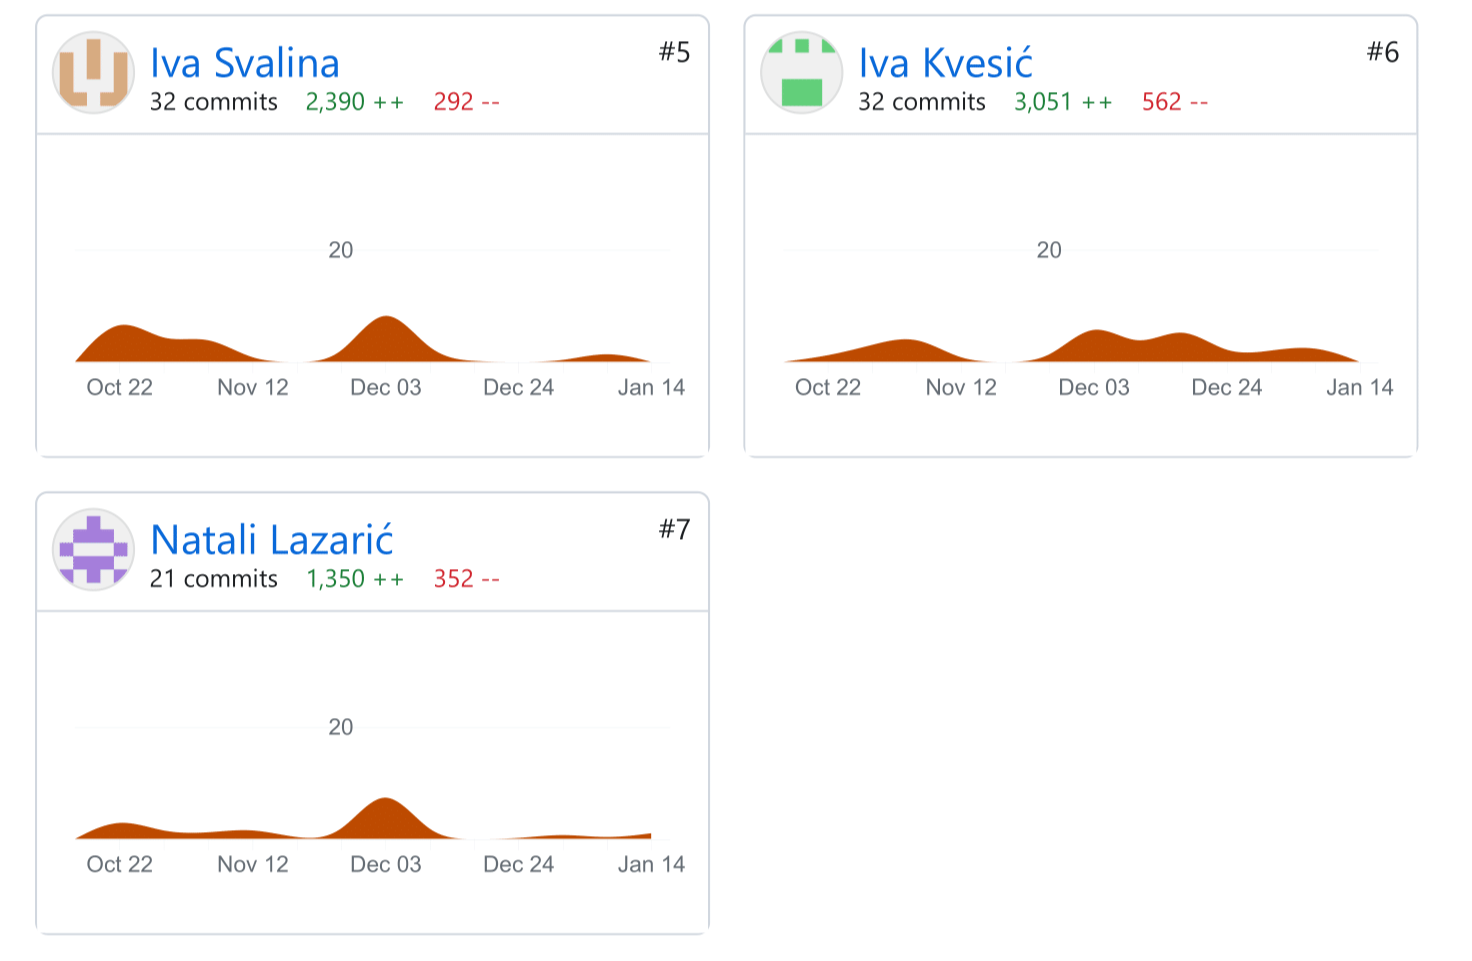
\includegraphics[width=\textwidth]{slike/promjene2.png}
			\centering
			\caption{Dijagram pregleda promjena, aktivnost na repozitoriju}
		\end{figure}
		
	


\end{document} %naredbe i tekst nakon ove naredbe ne ulaze u izgrađen dokument 


